\pdfoutput=1
\documentclass[11pt]{article}
\usepackage{jheppub}
\usepackage{epsfig}
\usepackage{amssymb}
\usepackage{amsmath}
\usepackage{tikz}
\usepackage{mathrsfs}
\usepackage{hyperref}
\usepackage{multirow}
\usepackage{scalerel}
\usepackage{mathtools}
\usepackage{textcomp}
\usepackage{color}
\usepackage[all]{xy}

\usetikzlibrary{calc}


\DeclareMathOperator{\B}{B}
\DeclareMathOperator{\Conf}{Conf}
\DeclareMathOperator{\Gr}{Gr}
\DeclareMathOperator{\Li}{Li}
\DeclareMathOperator{\sgn}{sgn}


\def\ket#1{\langle #1 \rangle}
\def\nl{\nonumber\\}
\def\nn{\nonumber}
\def\x{\mathcal{X}}
\def\xcoord{$\mathcal{X}$-coordinate }
\def\xcoords{$\mathcal{X}$-coordinates }
\def\a{\mathcal{A}}
\def\acoord{$\mathcal{A}$-coordinate }
\def\acoords{$\mathcal{A}$-coordinates }
\def\draftnote#1{{\bf [#1]}}
\def\flag{{\huge \color{red} \textinterrobang}}
\def\pdfeq#1{\texorpdfstring{$#1$}{a}}


\def\drawPentagon{
\coordinate (P1) at (90:1);
\coordinate (P2) at (18:1);
\coordinate (P3) at (306:1);
\coordinate (P4) at (234:1);
\coordinate (P5) at (162:1);
\draw (P1) -- (P2) -- (P3) -- (P4) -- (P5) -- cycle;
}

\def\drawLabeledPentagon{
\coordinate (P1) at (90:1);
\coordinate (P2) at (18:1);
\coordinate (P3) at (306:1);
\coordinate (P4) at (234:1);
\coordinate (P5) at (162:1);
\draw (P1) -- (P2) -- (P3) -- (P4) -- (P5) -- cycle;
\draw (0,1.2) node {1};
\draw (1,.3) node[anchor=west] {2};
\draw (.5,-.9) node[anchor=west] {3};
\draw (-.5,-.9) node[anchor=east] {4};
\draw (-1,.3) node[anchor=east] {5};
}

\def\drawOctagon{
\coordinate (P1) at (45:1);
\coordinate (P2) at (90:1);
\coordinate (P3) at (135:1);
\coordinate (P4) at (180:1);
\coordinate (P5) at (225:1);
\coordinate (P6) at (270:1);
\coordinate (P7) at (315:1);
\coordinate (P8) at (359:1);
\draw (P1) -- (P2) -- (P3) -- (P4) -- (P5) -- (P6) -- (P7) -- (P8) -- cycle;
}


\def\mand#1{\scaleto{s}{4.6pt}_{\scaleto{#1}{5.2pt}}}
\def\EthreeJ{{}^{{\{a,b\}}_3} {\cal E}_8}
\def\EfourJ{{}^{{\{a,b\}}_4} {\cal E}_8}
\def\LiOneCalX#1#2{\text{Li}_1(-\mathfrak{X}_{#1,#2})}
\def\LiOneBarCalX#1#2{\text{Li}_1(-\overline{\mathfrak{X}}_{#1,#2})}

\newcommand{\cP}{{\cal P}}
\def\lr{\leftrightarrow}

\title{Cluster Polylogarithms and Subalgebra-Constructibility\\ 
I \& II: Applications at 7 \& 8 Particles} 

\author{John~Golden$^{1,2}$}
\author{and Andrew~J.~McLeod$^{2,3,4}$}


\affiliation{$^1$ Leinweber  Center for Theoretical Physics and
Randall Laboratory of Physics, Department of Physics,
University of Michigan
Ann Arbor, MI 48109, USA}

\affiliation{$^2$ Kavli Institute for Theoretical Physics, 
UC Santa Barbara, Santa Barbara, CA 93106, USA}

\affiliation{$^3$ SLAC National Accelerator Laboratory,
Stanford University, Stanford, CA 94309, USA}

\affiliation{$^4$ Niels Bohr International Academy, Blegdamsvej 17, 2100 Copenhagen, Denmark}

\abstract{Everything we know about cluster algebras and polylogarithms.}


\begin{document}
\maketitle

\section{Pedantic introduction to cluster algebras}

Cluster algebras were introduced by Fomin and Zelevinsky \cite{1021.16017}, in large part motivated by questions of total positivity. The original goal was to gain a better understanding of what algebraic varieties can have a natural notion of positivity, and what functions can determine such positivity. A simple and highly-relevant example for amplitudes is the positive Grassmannian $\Gr^+(k,n)$, i.e. the space of $k\times n$ matrices where all ordered $k\times k$ minors are positive. 

What kind of questions can cluster algebras help us answer? One of the most straightforward is: how many minors do we need to specify a point in $\Gr^+(k,n)$? In other words, given a $k \times n$ matrix $M$, how many minors of $M$ do we have to calculate to know if $M \in \Gr^+(k,n)$? The reason that this is an interesting question is that the minors are not all independent, they satisfy the identities known as Pl\"ucker relations:
\begin{equation}
  \label{eq:plucker-rel}
  \ket{abI} \ket{cdI} = \ket{acI} \ket{bdI} + \ket{adI}\ket{bcI},
\end{equation}
where the Pl\"ucker coordinates = $\ket{i_1,\ldots,i_k}$ = the minor of columns $i_1, \ldots,i_k$, and $I$ is a multi-index with $k-2$ entries.

We'll now work through the example of $\Gr(2,5)$ in detail to try to understand how many minors one needs to check for positivity of the whole matrix. The 5 cyclically adjacent minors, $\ket{12}, \ket{23}, \ket{34}, \ket{45}, \ket{15}> 0$, are all independent from each other and so must each be checked. How many of the non-adjacent minors do we have to check? It turns out that the answer is 2. For example, if we specify that $\ket{13}, \ket{14}>0$ then we can use Pl\"ucker relations to show
\begin{equation}
\begin{split}
	\ket{24} &= (\ket{12}\ket{34} + \ket{23}\ket{14})/\ket{13}\\
	\ket{25} &= (\ket{12}\ket{45} + \ket{24}\ket{15})/\ket{14}\\
	\ket{35} &= (\ket{25}\ket{34} + \ket{23}\ket{45})/\ket{24}.
\end{split}	 	
\end{equation} 
Here we have expressed all of the remaining minors as sums and products of the cyclically adjacent minors along with $\ket{13}$ and $\ket{14}$, so everything is positive. 

So we only need to check two -- but can we check any two? Clearly we can use any of the cyclic images of $\{\ket{13}, \ket{14}\}$. What about $\{\ket{13}, \ket{25}\}$? This is a bit harder to see, but no, this pair does not work: there is no way to write down the remaining Pl\"uckers in terms of $\ket{13}$ and $\ket{25}$ such that everything is manifestly positive. For example, the matrix
\begin{equation}
\left(
\begin{array}{ccccc}
 1 & -1 & -4 & 3 & -2 \\
 2 & 2 & -6 & 4 & -1 \\
\end{array}
\right)
\end{equation}
satisfies $\ket{12},\ldots,\ket{15},\ket{13},\ket{25}>0$ but has $\ket{14},\ket{24},\ket{35}<0$. In the end, $\{\ket{13}, \ket{14}\}$ and its cyclic images are the only pairs that describe a point in $\Gr^+(2,5)$. 

This was easy enough to work out for this small case, but the problem gets much more complicated for larger matrices. However, there is a closely related, and much simpler, problem in geometry which can give us a bit more intuition: triangulating polygons.

Consider the following triangulation of the pentagon:
\begin{equation}
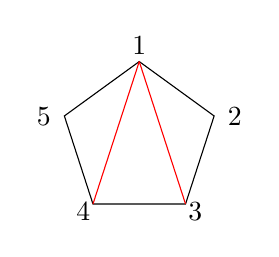
\begin{tikzpicture}
  \drawLabeledPentagon
  \draw[color=red] (P1) -- (P3);
  \draw[color=red] (P1) -- (P4);
\end{tikzpicture}
\end{equation}
We can immediately see the parallels with our $\Gr(2,5)$ situation (this is an example of the more general Pl\"ucker embedding which connects $\Gr(k,n)$ with projective space). Here we associate lines connecting points $i$ and $j$ with the Pl\"ucker coordinate $\ket{ij}$, and we see that the triangulations of the pentagon all describe points in $\Gr^+(2,5)$. In fact this correspondence holds between $n$-gons and $\Gr(2,n)$. 

A simple observation, but one at the very heart of cluster algebras, is that given some triangulation of a polygon one can create a \emph{new} triangulation by picking a quadrilateral and flipping its diagonal. For example:
\begin{equation}
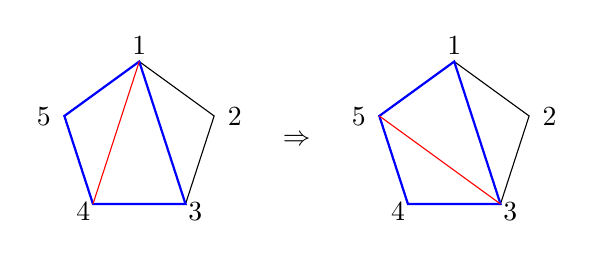
\begin{tikzpicture}
  \drawLabeledPentagon
  \draw[color=blue, thick] (P1) -- (P3) -- (P4) -- (P5) -- cycle;
  \draw[color=red] (P1) -- (P4);
  \draw (2,0) node {$\Rightarrow$};
\begin{scope}[xshift = 4cm]
  \drawLabeledPentagon
  \draw[color=blue, thick] (P1) -- (P3) -- (P4) -- (P5) -- cycle;
  \draw[color=red] (P5) -- (P3);
\end{scope}
\end{tikzpicture} 
\end{equation}
By repeatedly performing these flips one can generate all possible triangulations of a polygon:
\pagebreak
\begin{figure}[h!]
  \centering
  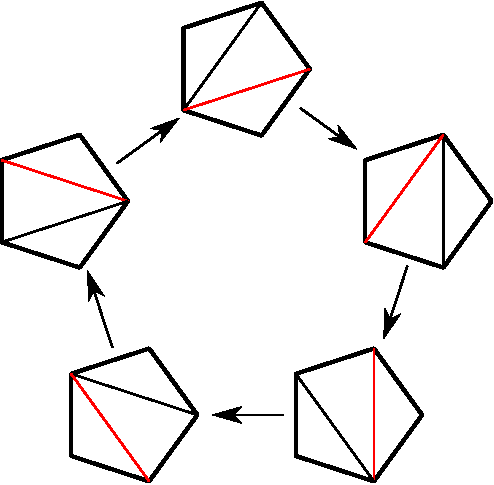
\includegraphics[scale=0.6]{pentagon-triangulations}
\end{figure}

\noindent where in each case the red diagonal gets flipped. 

Cluster algebras are a combinatorial tool which captures all of this structure (and much more!). The basic idea is that a cluser algebra is a collection of \emph{clusters}, which in this case represent individual triangulations of an $n$-gon, and these clusters are connected via a process called \emph{mutation}, which in this case is the flipping-the-diagonal process. We will initially describe everything in terms of Grassmannian cluster algebras, but the framework is entirely generalizable to other contexts of interest.

\subsubsection*{Basic definition}

We'll begin by constructing the cluster algebra for $\Gr(2,5)$. Each cluster is labeled by a collection of coordinates, which in this case are the edges of the pentagon along with the diagonals of the particular triangulation. These coordinates are then connected via an orientation of the pentagon and all subtriangles, for example:
\begin{equation}\label{eq:oriented-pentagon}
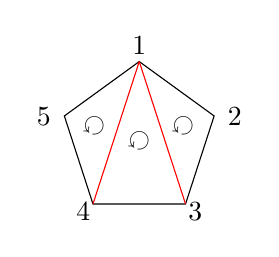
\begin{tikzpicture}
  \drawLabeledPentagon
  \draw[color=red] (P1) -- (P3);
  \draw[color=red] (P1) -- (P4);
  \draw (18:.6) node[rotate=144] {$\circlearrowleft$};
  \draw (0:0) node[rotate=144] {$\circlearrowleft$};
  \draw (162:.6) node[rotate=144] {$\circlearrowleft$};
\end{tikzpicture} 
\end{equation}
We can redraw this diagram as
\begin{equation}\label{eq:gr25-seed}
\begin{gathered}
\begin{xy} 0;<1pt,0pt>:<0pt,-1pt>::
	(25,25) *+{\langle 13\rangle} ="0",
	(75,25) *+{\langle 14\rangle} ="1",
	(125,25) *+{\framebox[5ex]{$\langle 15\rangle$}} ="2",
	(125,75) *+{\framebox[5ex]{$\langle 45\rangle$}} ="3",
	(75,75) *+{\framebox[5ex]{$\langle 34\rangle$}} ="4",
	(25,75) *+{\framebox[5ex]{$\langle 23\rangle$}} ="5",
	(0,0) *+{\framebox[5ex]{$\langle 12\rangle$}} ="6",
	(145,75) *+{},
	"0", {\ar"1"},
	"4", {\ar"0"},
	"0", {\ar"5"},
	"6", {\ar"0"},
	"1", {\ar"2"},
	"3", {\ar"1"},
	"1", {\ar"4"},
\end{xy}
\end{gathered}
\end{equation}
In this quiver diagram, we have an arrow between two Pl\"uckers $\ket{ab} \to \ket{cd}$ if the triangle orientations in eq. (\ref{eq:oriented-pentagon}) have segment $(ab)$ flowing into segment $(cd)$. The boxes around the $\ket{ii+1}$ indicate that they are \emph{frozen} -- in other words, we never change the outer edges of the pentagon, only the diagonal elements. And lastly it is unnecessary to draw the arrows connecting the outer edges, as that is redundant (and unchanging) information. 

We have now drawn our first cluster (also sometimes called a seed). To review/introduce some terminology, the Pl\"uckers are called cluster $\a$-coordinates (sometimes also $\a$-variables), and they come in two flavors: mutable ($\ket{13}$ and $\ket{14}$) and frozen ($\ket{ii+1}$). The information of the arrows can be represented in terms of a skew-symmetric adjacency matrix
\begin{equation}
	b_{i j} = (\# \text{arrows}\; i \to j) - (\# \text{arrows}\; j \to i).
\label{eq:bijdef}
\end{equation}

The process of mutation, which we described geometrically in terms of flipping the diagonal, has a simple interpretation at the level of this quiver. In particular, given a quiver such as eq. (\ref{eq:gr25-seed}), chose a node $k$ with associated $\a$-coordinate $a_k$ to mutate on (this is equivalent to picking which diagonal to flip). Then draw a new quiver that changes $a_{k}$ to $a_{k}'$ defined by
\begin{equation}
  \label{eq:mutation}
  a_{k} a_{k}' = \prod_{i \vert b_{i k} > 0} a_{i}^{b_{i k}} + \prod_{i \vert b_{i k} < 0} a_{i}^{-b_{i k}},
\end{equation} (with the understanding that an empty product is set to one) and leaves the other cluster coordinates unchanged. The arrows connecting the nodes in this new cluster are modified from the original cluster according to
\begin{itemize}
	\item for each path $i\to j \to k$, add an arrow $i\to j$,
	\item reverse all arrows on the edges incident with $k$,
	\item and remove any two-cycles that may have formed.
\end{itemize}
This creates a new adjacency matrix $b_{ij}'$ via 
\begin{equation}
  \label{eq:b-mutation}
  b'_{i j} =
  \begin{cases}
    -b_{i j}, &\quad \text{if $k \in \lbrace i, j\rbrace$,}\\
    b_{i j}, &\quad \text{if $b_{i k} b_{k j} \leq 0$,}\\
    b_{i j} + b_{i k} b_{k j}, &\quad \text{if $b_{i k}, b_{k j} > 0$,}\\
    b_{i j} - b_{i k} b_{k j}, &\quad \text{if $b_{i k}, b_{k j} < 0$.}
  \end{cases}
\end{equation}
Mutation is an involution, so mutating on $a_k'$ will take you back to the original cluster (as flipping the same diagonal twice will take you back to where you started). 

For our purposes, \emph{a cluster algebra is a set of quivers closed under mutation}. This means that mutating on any node of any quiver will generate a different quiver in the cluster algebra. The general procedure is to start with a quiver such as eq. (\ref{eq:gr25-seed}), with some collection of frozen and unfrozen nodes in a connected quiver, and continue mutating on all available nodes until you either close your set or convince yourself that the cluster algebra is infinite. 

We will end this brief introduction with a last piece of notation: cluster algebras are often referred to by particularly nice quiver types formed by their mutable nodes at some cluster. In the case of $\Gr(2,5)$, the mutable nodes of eq.~(\ref{eq:gr25-seed}) form an oriented $A_2$ Dynkin diagram, $\ket{13}\to\ket{14}$, and so we will often speak interchangeably of the cluster algebras for $\Gr(2,5)$ and $A_2$. This is a slight abuse of notation as the $\Gr(2,5)$ cluster algebra corresponds specifically to the cluster algebra generated by the collection of frozen and mutable nodes in eq.~(\ref{eq:gr25-seed}), whereas an $A_2$ cluster algebra is $a_1 \to a_2$ dressed with any number of frozen nodes. We will see how this language can be useful in the next section.

\subsection{Subalgebras}

Cluster algebras contain a rich and intricate subalgebra structure which will be critical for our upcoming physics applications. We can study a simple example by looking at triangulations of a hexagon, which is equivalently described by the cluster algebra associated with $\Gr(2,6)$:
\begin{equation}\label{eq:gr26-seed}
\begin{gathered}
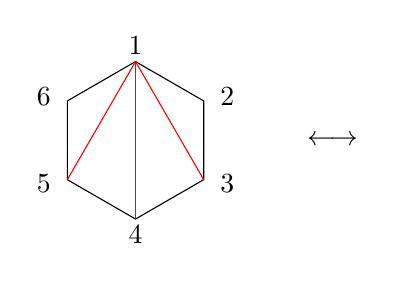
\begin{tikzpicture}
	\coordinate (P1) at (90:1);
	\coordinate (P2) at (30:1);
	\coordinate (P3) at (330:1);
	\coordinate (P4) at (270:1);
	\coordinate (P5) at (210:1);
	\coordinate (P6) at (150:1);
	\draw (P1) -- (P2) -- (P3) -- (P4) -- (P5) -- (P6) -- cycle;
  	\draw[color=red] (P1) -- (P3);
  	\draw[color=red] (P1) -- (P4);
  	\draw[color=red] (P1) -- (P5);
	\draw (0,1.2) node {1};
	\draw (30:1.1) node[anchor=west] {2};
	\draw (330:1.1) node[anchor=west] {3};
	\draw (270:1.2) node {4};
	\draw (210:1.1) node[anchor=east] {5};
	\draw (150:1.1) node[anchor=east] {6};
	\draw (2.5,0) node {$\longleftrightarrow$};
	\draw (3,0) node {\phantom{.}};
\end{tikzpicture} 
\begin{xy} 0;<1pt,0pt>:<0pt,-1pt>::
	(-50,-50) *+{\langle 13\rangle} ="13",
	(0,-50) *+{\langle 14\rangle} ="14",
	(50,-50) *+{\langle 15\rangle} ="15",
	(100,-50) *+{\framebox[5ex]{$\langle 16\rangle$}} ="16",
	(100,0) *+{\framebox[5ex]{$\langle 56\rangle$}} ="56",
	(50,0) *+{\framebox[5ex]{$\langle 45\rangle$}} ="45",
	(0,0) *+{\framebox[5ex]{$\langle 34\rangle$}} ="34",
	(-50,0) *+{\framebox[5ex]{$\langle 23\rangle$}} ="23",
	(-75,-75) *+{\framebox[5ex]{$\langle 12\rangle$}} ="12",
	(70,0) *+{},
	"12", {\ar"13"},
	"13", {\ar"14"},
	"13", {\ar"23"},
	"34", {\ar"13"},
	"14", {\ar"15"},
	"14", {\ar"34"},
	"45", {\ar"14"},
	"15", {\ar"45"},
	"56", {\ar"15"},
	"15", {\ar"16"},
\end{xy}
\end{gathered}
\end{equation}
The cluster algebra associated with $\Gr(2,6)$ features 14 clusters, and these clusters can be grouped together in to multiple (overlapping) sets which we call subalgebras. A simple example is the collection of all triangulations which involve the cord $\ket{15}$. This set is itself a cluster algebra, and can be generated via mutations by taking the diagram in eq.~(\ref{eq:gr26-seed}), ``freezing'' the cord $\ket{15}$, then mutating on the other two cords. This of course is just the cluster algebra of triangulating a pentagon
\begin{equation}
\begin{gathered}
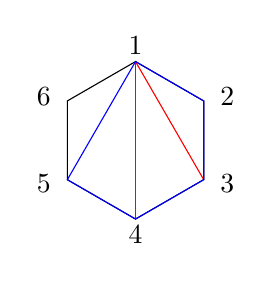
\begin{tikzpicture}
	\coordinate (P1) at (90:1);
	\coordinate (P2) at (30:1);
	\coordinate (P3) at (330:1);
	\coordinate (P4) at (270:1);
	\coordinate (P5) at (210:1);
	\coordinate (P6) at (150:1);
	\draw (P1) -- (P2) -- (P3) -- (P4) -- (P5) -- (P6) -- cycle;
  	\draw[color=red] (P1) -- (P3);
  	\draw[color=red] (P1) -- (P4);
	\draw[color=blue] (P1) -- (P2) -- (P3) -- (P4) -- (P5) -- cycle;
	\draw (0,1.2) node {1};
	\draw (30:1.1) node[anchor=west] {2};
	\draw (330:1.1) node[anchor=west] {3};
	\draw (270:1.2) node {4};
	\draw (210:1.1) node[anchor=east] {5};
	\draw (150:1.1) node[anchor=east] {6};
\end{tikzpicture} 
\end{gathered}
\end{equation}
 


\subsection{An overview of finite cluster algebras}\label{sec:finite-algebras}
Fortunately, Fomin and Zelevinksy classified all finite cluster algebras in\cite{1054.17024}. In particular, they showed that a cluster algebra is of finite type iff the mutable part of its quiver at some cluster takes the form of an oriented, simply-laced Dynkin diagram: $A_n, D_n, E_{n\le8}$. We will describe several of the relevant cases to give the reader a flavor for the world of finite algebras. 

Cluster algebras of type $A_n$ 
\begin{equation}\label{def:An}
  x_1\to x_2\to \ldots \to x_n
\end{equation}
correspond to triangulations of an $(n+3)$-gon, where each cluster is a triangulation, each \acoord is a cord, and each \xcoord is a quadrilateral with a cord as a diagonal embedded in the $(n+3)$-gon. This makes the counting easy: the number of clusters for $A_n$ is given by the Catalan number $C(n+1)$, the number of \acoords is $\binom{n+3}{2}-n$, and the number of \xcoords is $2\binom{n+3}{4}$. Subalgebras correspond to embedding a smaller polygon in to the $(n+3)$-gon, for example the $A_2$ subalgebras in $A_5$ are the $56=\binom{8}{5}$ pentagonal embeddings in an octagon. 

The cluster algebra $D_4$
\begin{equation}\label{def:D4}
    \begin{gathered}
    \begin{xy} 0;<1pt,0pt>:<0pt,-1pt>::
      (0,20) *+{x_1} ="1",
      (30,20) *+{x_2} ="2",
      (60,0) *+{x_3} ="3",
      (60,40) *+{x_4} ="4",
      "1", {\ar"2"},
      "2", {\ar"3"},
      "2", {\ar"4"},
    \end{xy}
    \end{gathered}
\end{equation}
has 50 clusters, 16 \acoords, and 104 \xcoords. There are 36 $A_2$ subalgebras and 12 $A_3$ subalgebras. 

The cluster algebra $D_5$
\begin{equation}\label{def:D5}
    \begin{gathered}
    \begin{xy} 0;<1pt,0pt>:<0pt,-1pt>::
      (0,20) *+{x_1} ="1",
      (30,20) *+{x_2} ="2",
      (60,20) *+{x_3} ="3",
      (90,0) *+{x_4} ="4",
      (90,40) *+{x_5} ="5",
      "1", {\ar"2"},
      "2", {\ar"3"},
      "3", {\ar"4"},
      "3", {\ar"5"},
    \end{xy}
    \end{gathered}
\end{equation}
has 182 clusters, 25 \acoords, and 260 \xcoords. There are 125 distinct $A_2$ subalgebras, 65 $A_3$, 10 $A_4$, and 5 $D_4$. 

Finally, we describe the cluster algebra $E_6$
\begin{equation}\label{def:E6}
    \begin{gathered}
    \begin{xy} 0;<1pt,0pt>:<0pt,-1pt>::
      (0,0) *+{x_1} ="1",
      (30,0) *+{x_2} ="2",
      (60,0) *+{x_3} ="3",
      (60,-25) *+{x_4} ="4",
      (90,0) *+{x_5} ="5",
      (120,0) *+{x_5} ="6",
      "1", {\ar"2"},
      "2", {\ar"3"},
      "4", {\ar"3"},
      "5", {\ar"3"},
      "6", {\ar"5"},
    \end{xy}
    \end{gathered}
\end{equation}
which has 833 clusters, 42 \acoords, and 770 \xcoords. The subalgebra counting is: 
\begin{equation}
\begin{tabular}{ c|c|c|c|c|c} 
 $A_2$ & $A_3$ & $A_4$ & $D_4$ & $A_5$ & $D_5$ \\ 
 \hline
504 & 364 & 98 & 35 & 7 & 14
\end{tabular}.
\end{equation}

\subsection{Cluster automorphisms}

See \cite{Chang:2015} for a more thorough mathematical introduction. The simplest example of a cluster automorphism is what we will call a direct automorphism. Let $\a$ be a cluster algebra. Then $f: \a \to \a$ is direct automorphism of $\a$ if
\begin{itemize}
  \item for every cluster $\mathbf{x}$ of $\a$, $f(\mathbf{x})$ is also a cluster of $\a$,
  \item $f$ respects mutations, i.e. $f(\mu(x_i,\mathbf{x})) = \mu(f(x_i),f(\mathbf{x}))$.
 \end{itemize} 
A simple example of this for $A_2$ is the map
\begin{equation}
  \sigma_{A_2}:\quad \mathcal{X}_i \to \mathcal{X}_{i+1},
\end{equation}
which cycles the five clusters $1/\x_i\to \x_{i+1}$ amongst themselves, and can be cast in terms of the seed variables $x_1, x_2$ as 
\begin{equation}
  \sigma_{A_2}:\quad x_1\to \frac{1}{x_2},~~ x_2\to x_1(1+x_2).
\end{equation}

A less obvious example of a cluster automorphism is what are called indirect automorphisms, which respect mutations but do not map clusters directly on to clusters; instead
\begin{itemize}
  \item for every cluster $\mathbf{x}$ of $\a$, $f(\mathbf{x})$ + invert all nodes + swap direction of all arrows\\ = a cluster of $\a$.
\end{itemize}
For $A_2$ we have the indirect automorphism
\begin{equation}
  \tau_{A_2}:\quad \mathcal{X}_i \to \mathcal{X}_{6-i},
\end{equation}
where indices are understood to be mod 5, and can instead be cast in terms of the seed variables $x_1, x_2$ as
\begin{equation}
  \tau_{A_2}:\quad x_1 \to \frac{1}{x_2}, ~~x_2 \to \frac{1}{x_1}.
\end{equation}
We can see how this works in a simple example
\begin{align}
  \tau_{A_2}(1/\x_1 \to \x_2) =&~1/\x_5 \to \x_4 \nl
  \Rightarrow &\text{ invert each node and swap direction of all arrows }\\ 
  =&~\x_5 \leftarrow 1/\x_4, \text{ which is in the original $A_2$}.\nn
\end{align}
It is useful to think of indirect automorphisms as generating a ``mirror'' or ``flipped'' version of the original $\a$, where the total collection of $\x$-coordinates is the same, but their Poisson bracket has flipped sign. The existence of this flip then can be seen as resulting from the choice of assigning $b_{ij}$ = (\# arrows $i\to j$) - (\# arrows $j \to i$), where instead we could have chosen $b_{ij}$ = (\# arrows $j \to i$) - (\# arrows $i\to j$) and still generated the same clsuter algebraic structure, albeit with different labels for the nodes. In the generic case this is an arbitrary choice, and $\tau$ captures the superficiality of the notation change.

The automorphisms $\sigma_{A_2}$ and $\tau_{A_2}$ generate the complete automorphism group for $A_2$, namely, $D_5$ (the notation here is regretably redundant; here we are referring to the dihedral group of five elements, which is of course distinct from the Dynkin diagram $D_5$ -- we hope that context will clarify to the reader what we mean in each case). We now list generators for the automorphism groups of the finite algebras discussed already. First we adopt the notation
\begin{equation}
	x_{i_1,\ldots, i_k} = \sum_{a=1}^k \prod_{b=1}^a x_{i_b} = x_{i_1}+x_{i_1}x_{i_2} + \ldots + x_{i_1}\cdots x_{i_k}.
\end{equation}

Cluster algebras of type $A_n$, as defined in eq.~(\ref{def:An}), have automorphism group $D_{n+3}$, with a cyclic generator $\sigma_{A_n}$ (direct, length $n+3$)
\begin{equation}
  \sigma_{A_n}:\quad x_{k<n} \to \frac{x_{k+1}(1+x_{1,\ldots,k-1})}{1+x_{1,\ldots,k+1}},~~x_n\to\frac{1+x_{1,\ldots,n-1}}{\prod_{i=1}^n x_i}
\end{equation}
and flip generator $\tau_{A_n}$ (indirect)
\begin{equation}
  \tau_{A_n}: \quad x_1 \to \frac{1}{x_n},~~x_2 \to \frac{1}{x_{n-1}},~\ldots~,x_n\to\frac{1}{x_1}.
\end{equation}


The cluster algebra $D_4 \simeq \Gr(3,6)$, as defined in eq.~(\ref{def:D4}), has automorphism group $D_4\times S_3$, with two cyclic generators: 
\begin{equation}
\begin{split}
  \sigma^{(4)}_{D_4}:\quad& 
    x_1\to\frac{x_2}{1+x_{1,2}},~~  
    x_2\to\frac{\left(1+x_1\right)x_1 x_2 x_3 x_4}{\left(1+x_{1,2,3}\right) \left(1+x_{1,2,4}\right)},~~
    x_3\to\frac{1+x_{1,2}}{x_1 x_2 x_3},~~
    x_4\to\frac{1+x_{1,2}}{x_1 x_2 x_4},\\ \\
  \sigma^{(3)}_{D_4}:\quad& 
    x_1\to \frac{1}{x_3},~~
    x_2\to \frac{x_1 x_2 \left(1+x_3\right)}{1+x_1},~~
    x_3\to x_4,~~
    x_4\to \frac{1}{x_1},
\end{split}  
\end{equation}
where $\sigma^{(4)}_{D_4}$ generates the 4-cycle and $\sigma^{(3)}_{D_4}$ the 3-cycle in $D_4$ and $S_3$, respectively. Then there is the indirect $\tau$-flip associated with the $D_4$ automorphism, as well as a direct $\mathbb{Z}_2$-flip associated with the $S_3$ automorphism:
\begin{equation}
\begin{split}
  \tau_{D_4}:\quad& 
    x_2\to \frac{1+x_1}{x_1 x_2 \left(1+x_3\right) \left(1+x_4\right)},\\ \\
  \mathbb{Z}_{2,D_4}:\quad& 
    x_3\to x_4,~~
    x_4\to x_3.
\end{split}  
\end{equation}
The cluster algebra $D_{n>4}$
\begin{equation}
    \begin{gathered}
    \begin{xy} 0;<1pt,0pt>:<0pt,-1pt>::
      (0,20) *+{x_1} ="1",
      (30,20) *+{x_2} ="2",
      (60,20) *+{\ldots} ="3",
      (90,20) *+{x_{n-2}} ="4",
      (120,0) *+{x_{n-1}} ="5",
      (120,40) *+{x_{n}} ="6",
      "1", {\ar"2"},
      "2", {\ar"3"},
      "3", {\ar"4"},
      "4", {\ar"5"},
      "4", {\ar"6"},
    \end{xy}
    \end{gathered}
\end{equation}
has automorphism group $D_n \times \mathbb{Z}_2$ with generators $\sigma_{D_n}$ ($n$-cycle, direct), $\mathbb{Z}_{2,D_n}$ (2-cycle, direct), and $\tau_{D_n}$ (2-cycle, indirect). The $Z_2$ simply swaps $x_{n-1} \leftrightarrow x_n$, and for $D_5$, as defined in eq.~(\ref{def:D5}), the $\sigma$ and $\tau$ generators can be represented by
\begin{equation}
\begin{split}
  \sigma_{D_5}:\quad& 
    x_1\to \frac{x_2}{1+x_{1,2}},~~
    x_2\to \frac{(1+x_1) x_3}{1+x_{1,2,3}},~~
    x_3\to \frac{x_1 x_2 x_3 x_4 x_5 (1+x_{1,2})}{(1+x_{1,2,3,4}) (1+x_{1,2,3,5})},\\&
    x_4\to \frac{1+x_{1,2,3}}{x_1 x_2 x_3 x_4},~~
    x_5\to \frac{1+x_{1,2,3}}{x_1 x_2 x_3 x_5},\\ \\
  \tau_{D_5}:\quad& 
    x_1\to x_1,~~
    x_2\to \frac{1+x_1}{x_1 x_2 (1+x_3 x_5+x_{3,4,5})},~~
    x_3\to \frac{x_3 x_4 x_5}{(1+x_{3,4}) (1+x_{3,5})},\\&
    x_4\to \frac{1+x_3 x_5+x_{3,4,5}}{x_4},~~
    x_5\to \frac{1+x_3 x_5+x_{3,4,5}}{x_5}.
\end{split}  
\end{equation}
$E_6 \simeq \Gr(4,7)$, as defined in eq.~(\ref{def:E6}), has automorphism group $D_{14}$ with generators $\sigma_{E_6}$ (7-cycle, direct), $\mathbb{Z}_{2,E_6}$ (2-cycle, direct), and $\tau_{E_6}$ (2-cycle, indirect). In $\Gr(4,7)$ language, these are the traditional cycle ($Z_i \to Z_{i+1}$), parity ($Z \to W$'s), and flip ($Z_i \to Z_{8-i}$) symmetries, respectively. In $E_6$ language they can be represented by 
\begin{equation}
\begin{split}
  \sigma_{E_6}:\quad& 
    x_1\to \frac{1}{x_6 (1+x_{5,3,4})},~~
    x_2\to \frac{1+x_{6,5,3,4}}{x_5 (1+x_{3,4})},~~
    x_3\to \frac{(1+x_{2,3,4}) (1+x_{5,3,4})}{x_3 (1+x_4)},\\&
    x_4\to \frac{1+x_{3,4}}{x_4},~~
    x_5\to \frac{1+x_{1,2,3,4}}{x_2 (1+x_{3,4})},~~
    x_6\to \frac{1}{x_1 (1+x_{2,3,4})},\\ \\
  \mathbb{Z}_{2,E_6}:\quad& 
    x_i\to x_{7-i},\\ \\
  \tau_{E_6}:\quad& 
    x_1\to \frac{x_5}{1+x_{6,5}},~~
    x_2\to (1+x_5) x_6,~~
    x_3\to \frac{(1+x_{1,2}) (1+x_{6,5})}{x_1 x_2 x_3 x_5 x_6 (1+x_4)},\\&
    x_4\to x_4,~~
    x_5\to x_1 (1+x_2),~~
    x_6\to \frac{x_2}{1+x_{1,2}}.
\end{split}  
\end{equation}

\subsection{Associahedra}

Understanding the way in which clusters are related to each other via mutation is a hot topic of research. A sample question is: given two clusters in the same cluster algebra, what is the minimal set of mutations necessary to get from one cluster to the other? While I don't delve in to this area too much, I do want to give an introduction to a relevant and important object associated with a cluster algebra: the associahedron (often also called the Stasheff polytope). The basic idea is to create a graph where the nodes are clusters and edges are drawn between clusters connected via mutation. So the figure
\begin{figure}[h]
  \centering
  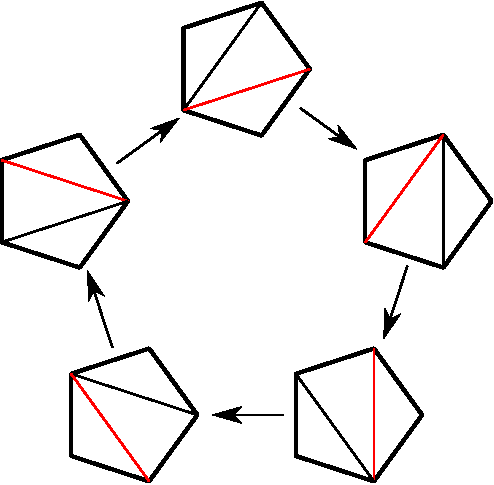
\includegraphics[scale=0.6]{pentagon-triangulations}
\end{figure}

is in fact the $\Gr(2,5)$ or $A_2$ associahedron, and clearly it takes the form of a pentagon (one should ignore the orientation on the edges of the pentagon).

The associahedron associated with the $\Gr(2,6) \leftrightarrow A_3$ cluster algebra (i.e. triangulations of a hexagon) is
\begin{figure}[h]
  \centering
  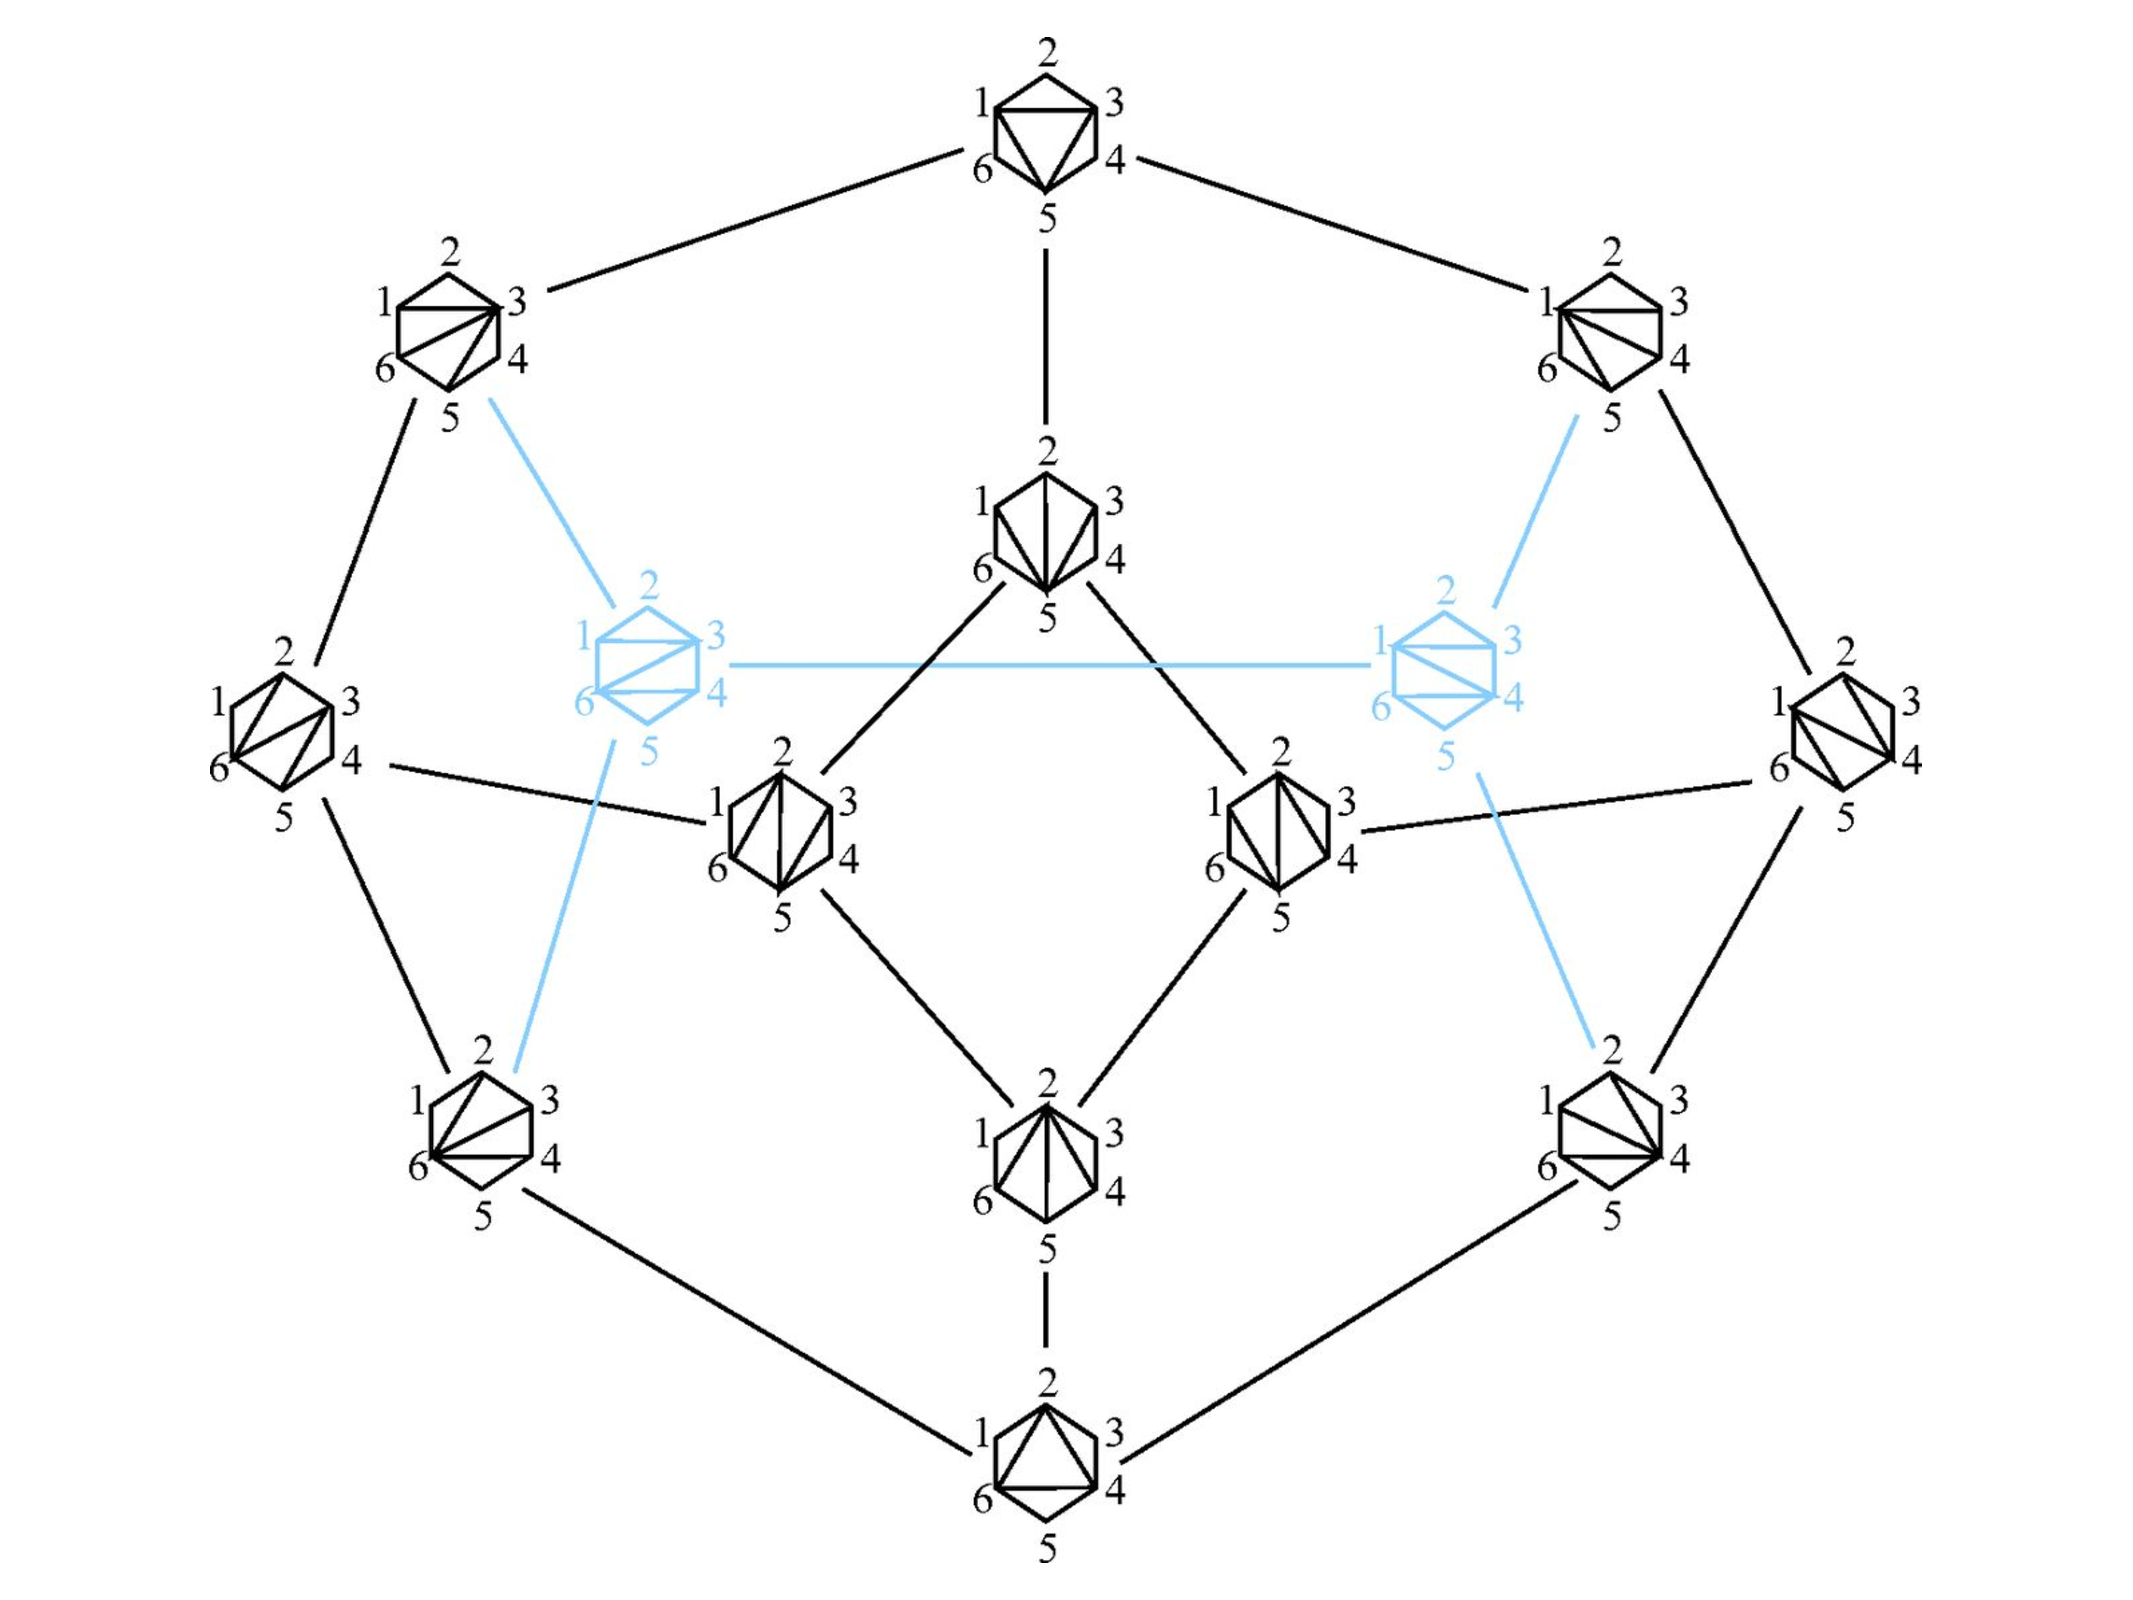
\includegraphics[scale=0.25]{a3-associahedron}
\end{figure}

This associahedron has 14 vertices, with 3 square faces and 6 pentagonal faces. Because of the Grassmannian duality $\Gr(2,6) = \Gr(4,6)$, this (remarkably simple!) cluster algebra and associahedron play an integral role in the momentum twistors for 6-particle kinematics for $\mathcal{N}=4$ SYM. 

$\Gr(4,7) \leftrightarrow E_6$, which is associated with 7-particle momentum twistors, is a bit more complicated: it features 833 clusters, and the associahedron is a polytope with nodes of valence 6. The dimension-2 faces are 1785 squares and 1071 pentagons, and there are 49 different $A$-coordinates that appear. The associahedron looks like
\begin{figure}[h]
  \centering
  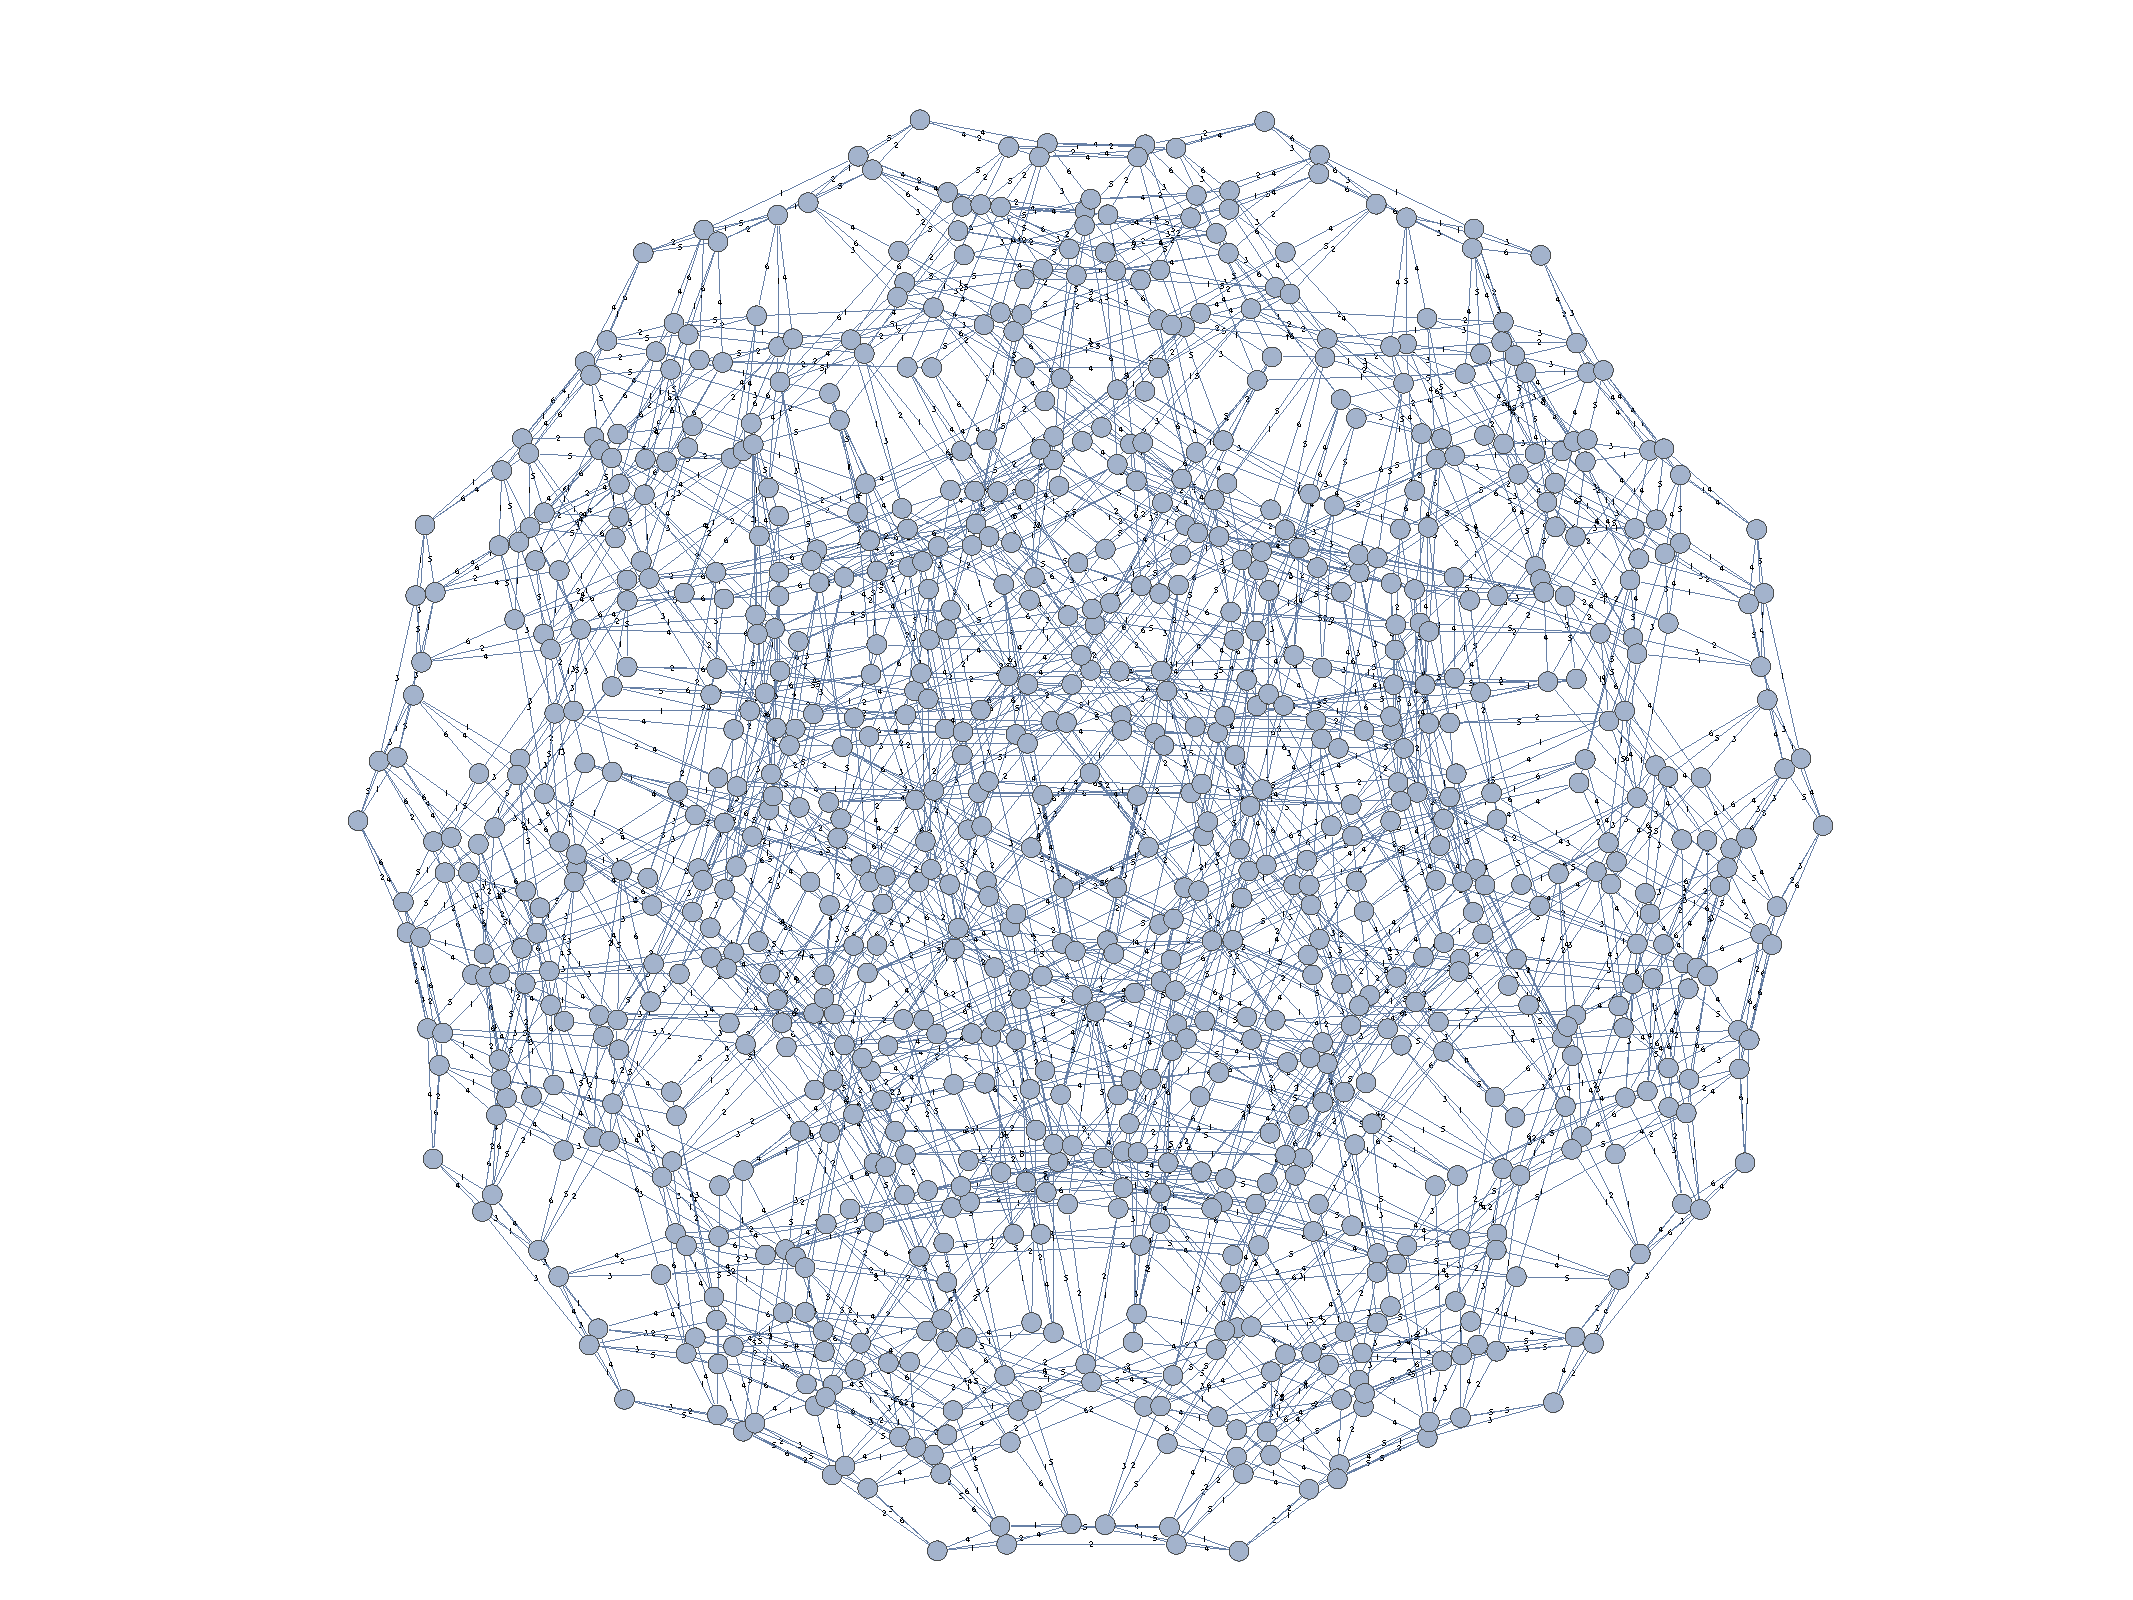
\includegraphics[scale=0.25]{e6-associahedron}
\end{figure}


It is not important to memorize any of this -- I just want to give you a flavor for the rich and complex structures that can arise from the simple mutation rules of eq. (\ref{eq:mutation})!

\subsection{Grassmannian cluster algebras (and cluster Poisson spaces)}
For $\Gr(k,n)$, Scott showed \cite{1088.22009} that the associated seed cluster is
\begin{center}
\begin*{}
\begin{xy} 0;<.5pt,0pt>:<0pt,-.5pt>::
(0,0) *+{f_{1 l}} ="0",
(75,0) *+{\cdots} ="1",
(150,0) *+{f_{13}} ="2",
(225,0) *+{f_{12}} ="3",
(300,0) *+{\framebox[5ex]{$f_{11}$}} ="4",
(0,75) *+{f_{2 l}} ="5",
(75,75) *+{\cdots} ="6",
(150,75) *+{f_{23}} ="7",
(225,75) *+{f_{22}} ="8",
(300,75) *+{\framebox[5ex]{$f_{21}$}} ="9",
(0,150) *+{\vdots} ="10",
(75,150) *+{\vdots} ="11",
(150,150) *+{\vdots} ="12",
(225,150) *+{\vdots} ="13",
(300,150) *+{\vdots} ="14",
(0,225) *+{\framebox[5ex]{$f_{kl}$}} ="15",
(75,225) *+{\cdots} ="16",
(150,225) *+{\framebox[5ex]{$f_{k3}$}} ="17",
(225,225) *+{\framebox[5ex]{$f_{k2}$}} ="18",
(300,225) *+{\framebox[5ex]{$f_{k1}$}} ="19",
(-60,0) *+{} ="20",
"0", {\ar"1"},
"0", {\ar"5"},
"6", {\ar"0"},
"1", {\ar"2"},
"2", {\ar"3"},
"2", {\ar"7"},
"8", {\ar"2"},
"3", {\ar"4"},
"3", {\ar"8"},
"9", {\ar"3"},
"5", {\ar"6"},
"5", {\ar"10"},
"6", {\ar"7"},
"7", {\ar"8"},
"7", {\ar"12"},
"13", {\ar"7"},
"8", {\ar"9"},
"8", {\ar"13"},
"14", {\ar"8"},
"10", {\ar"15"},
"12", {\ar"17"},
"19", {\ar"13"},
"18", {\ar"12"},
"13", {\ar"18"},
\end{xy}
\end*{}
\end{center}

where
\begin{equation}
  f_{i j} =
  \begin{cases}
    \frac {\langle i+1, \dotsc, k, k+j, \dotsc, i+j+k-1\rangle}{\langle 1, \dotsc, k\rangle}, \qquad &i \leq l-j+1,\\
    \frac {\langle 1, \dotsc, i+j-l-1, i+1, \dotsc, k, k+j, \dotsc, n\rangle}{\langle 1, \dotsc, k\rangle}, \qquad &i > l-j+1
  \end{cases},
\end{equation}
We can use this to find the Grassmannian cluster algebras of finite type, they are:
\begin{equation}
	\Gr(2,n) \leftrightarrow A_{n-3}, \quad \Gr(3,6) \leftrightarrow D_4, \quad \Gr(4,7) \leftrightarrow E_6, \quad \Gr(3,8) \leftrightarrow E_8.
\end{equation}
An intriguing point for those of us studying $\mathcal{N}=4$ SYM, where the momentum twistors describing particle kinematics live in $\Gr(4,n)$, is that only $\Gr(4,n<8)$ are finite. The ramifications of the fact that $n>7$-particle kinematics are associated with infinite cluster algebras are still being worked out. 

Another important set of information encoded in cluster algebras are called Fock-Goncharov or $\x$-coordinates. Given a quiver described by the matrix $b$, the $\a$- and $\x$-coordinates are related as follows:
\begin{equation}
	x_i = \prod_j a_j^{b_{ij}}. 	
\end{equation} 
For example, the quiver 
\begin{equation}
\begin{gathered}
\begin{xy} 0;<1pt,0pt>:<0pt,-1pt>::
	(25,25) *+{\langle 13\rangle} ="0",
	(75,25) *+{\langle 14\rangle} ="1",
	(125,25) *+{\framebox[5ex]{$\langle 15\rangle$}} ="2",
	(125,75) *+{\framebox[5ex]{$\langle 45\rangle$}} ="3",
	(75,75) *+{\framebox[5ex]{$\langle 34\rangle$}} ="4",
	(25,75) *+{\framebox[5ex]{$\langle 23\rangle$}} ="5",
	(0,0) *+{\framebox[5ex]{$\langle 12\rangle$}} ="6",
	(145,75) *+{},
	"0", {\ar"1"},
	"4", {\ar"0"},
	"0", {\ar"5"},
	"6", {\ar"0"},
	"1", {\ar"2"},
	"3", {\ar"1"},
	"1", {\ar"4"},
\end{xy}
\end{gathered}
\end{equation}
has $\x$-coordinates 
\begin{equation}\label{def:xcoordsA2}
	\x_1 = \frac{\ket{12}\ket{34}}{\ket{14}\ket{23}}, \quad \x_2 = \frac{\ket{13}\ket{45}}{\ket{15}\ket{34}}.
\end{equation}
In the pentagon-triangulation picture, these $\x$-coordinates describe overlapping quadrilaterals:
\begin{center}
\begin{equation}
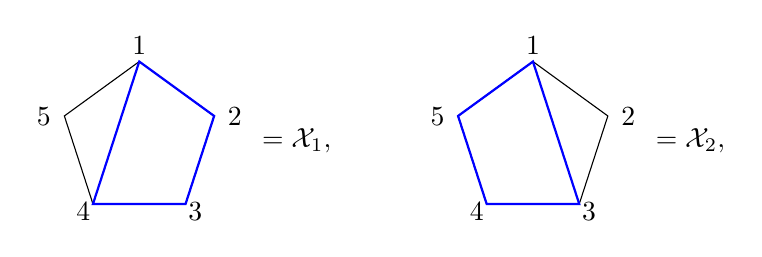
\begin{tikzpicture}
  \drawLabeledPentagon
  \draw[color=blue, thick] (P1) -- (P2) -- (P3) -- (P4) -- cycle;
  \draw (2,0) node {$=\x_1,$};
\begin{scope}[xshift = 5cm]
  \drawLabeledPentagon
  \draw[color=blue, thick] (P1) -- (P3) -- (P4) -- (P5) -- cycle;
  \draw (2,0) node {$=\x_2,$};
\end{scope}
\end{tikzpicture} 
\end{equation}
\end{center}
The nice feature of $\x$-coordinates, at least from a physicists perspective, is that in the case of $\Gr(4,n)$ the $\x$-coordinates are dual-conformal invariant cross-ratios. We can see this for example in the two-loop, six-particle remainder function for $\mathcal{N}=4$ SYM:
\begin{align}
	R^{(2)}_6 = &\sum_{\text{cyclic}} \text{Li}_4\left(-\frac{\langle 1234 \rangle \langle 2356 \rangle}{\langle 1236 \rangle \langle 2345 \rangle}\right) - \frac{1}{4} \text{Li}_4 \left(-\frac{\langle 1246 \rangle \langle 1345 \rangle}{\langle 1234 \rangle \langle 1456 \rangle}\right)\nl
	&+\text{products of } \text{Li}_{k}(-x) \text{ functions of lower weight}\\ &\quad~\text{with the same set of arguments.}\nn
\end{align}
The arguments of the polylogarithms all take the form of $(-\x)$-coordinates for $\Gr(4,6)$. $\x$-coordinates play other important roles in the context of polylogarithm functions independent of scattering amplitudes, for example with $\Gr(2,5) \leftrightarrow A_2$ we have 
\begin{equation}
	\sum_\text{cyclic} \Li_2(-\x_i) + \log(\x_i)\log(\x_{i+1}) = \frac{\pi^2}{6}
\end{equation}
where the definition of $\x_i$ can be inferred from eq. (\ref{def:xcoordsA2}). There are more complicated examples of polylogarithm identities satisfied by groups of $\x$-coordinates, for example there is a 40-term identity among $\Li_3$ functions where all of the arguments are $(-\x)$

Since we are motivated from physics to cast our final function-level results in terms of $\x$-coordinates it is useful to work entirely in that language rather than the $\a$-coordinates. The mutation rules for the $\x$-coordinates are
\begin{equation}
  \label{eq:x-coords-mutation}
  x_{i}' =
  \begin{cases}
    x_{k}^{-1}, &\quad i=k,\\
    x_{i} (1+x_{k}^{\sgn b_{i k}})^{b_{i k}}, &\quad i \neq k
  \end{cases},
\end{equation}
and the adjacency matrix $b_{ij}$ changes following eq.~(\ref{eq:b-mutation}). From here on out we will write our quivers entirely in terms of $\x$-coordinates, for example $A_2$ is 
\begin{equation}
	x_1 \to x_2.
\end{equation}
By continuing to mutate on alternating nodes (denoted below by \mbox{\color{red}{red}}) we generate the following sequence of clusters:
\begin{align}
  x_1 &\to \color{red}{x_2} \nl
  \color{red}{x_1(1+x_2)} &\leftarrow \frac{1}{x_2} \nl
  \frac{1}{x_1(1+x_2)} &\to \color{red}{\frac{x_2}{1+x_1+x_1 x_2}} \\
  \color{red}{\frac{x_1 x_2}{1+x_1}} &\leftarrow \frac{1+x_1+x_1 x_2}{x_2} \nl
  \frac{1+x_1}{x_1 x_2} &\to \color{red}{\frac{1}{x_1}} \nl
  \color{red}{x_2} &\leftarrow x_1 \nl
  &\vdots \nn
\end{align}
where the series then repeats. Note that by labeling the $\x$-coordinates as
\begin{equation}\label{def:a2-xcoords}
  \x_1 = 1/x_1, \quad \x_2 = x_2, \quad \x_3 = x_1(1+x_2), \quad 
  \x_4 = \frac{1+x_1+x_1 x_2}{x_2}, \quad \x_5 = \frac{1+x_1}{x_1 x_2},
\end{equation}
then the general mutation rule of eq. (\ref{eq:x-coords-mutation}) takes the simple form of
\begin{equation}\label{eq:exchange-relation}
  1+\x_i = \x_{i-1}\x_{i+1}.
\end{equation}
Putting this all together, we say that an $A_2$ cluster algebra is any set of clusters $1/\x_{i-1} \to \x_i$ for $i=1\ldots5$ where the $\x_i$ satisfy eq. (\ref{eq:exchange-relation}). We believe it is useful at this point to emphasize that one can take as input any $\{x_1, x_2\}$ and generate an associated $A_2$. For example, one could start with the quiver $3\to\frac{7}{2}$ and generate the $A_2$
\begin{equation}
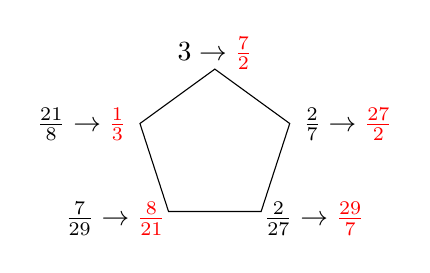
\begin{tikzpicture}
  \drawPentagon
  \draw (0,1.2) node {$3\to\color{red}{\frac{7}{2}}$};
  \draw (1,.3) node[anchor=west] {$\frac{2}{7} \to \color{red}{\frac{27}{2}} $};
  \draw (.5,-.9) node[anchor=west] {$\frac{2}{27} \to \color{red}{\frac{29}{7}}$};
  \draw (-.5,-.9) node[anchor=east] {$\frac{7}{29} \to \color{red}{\frac{8}{21}}$};
  \draw (-1,.3) node[anchor=east] {$\frac{21}{8} \to \color{red}{\frac{1}{3}}$};
\end{tikzpicture}
\end{equation}
(Mutating on the node in red moves you clockwise around the pentagon.) In future sections it will be necessary to consider collections of multiple $A_2$ algebras, in such cases we label them by only one of their clusters, e.g. $x_1 \to x_2$, with the understanding that we are referring to the $A_2$ which contains that cluster as an element. 

\subsubsection{Applications to momentum twistors and \pdfeq{\mathcal{N}}=4 SYM}

\section{Cluster polylogarithms}
\subsection{Lie cobracket and motivic content}
\subsubsection{Review of previous results}
\subsection{Cluster adjacency}
Cluster adjacency is a property of all Steinmann-satisfying amplitudes, and was first introduced in \cite{Drummond:2017ssj}. The original phrasing of this property is that the symbol of all Steinmann-satisfying integrals in $n$-particle kinematics, when fully expanded out in terms of \acoords, is of the form 
\begin{equation}
	\ldots \otimes \alpha_i \otimes \alpha_j\otimes \ldots 
\end{equation}
where $\alpha_i$ and $\alpha_j$ appear together in a cluster of $\Gr(4,n)$. This non-trivial property is a considerable constraint on the space of polylogarithm functions which can appear in amplitudes. 

The original presentation of cluster adjacency was in terms of \acoords, but adjacency can also be phrased in terms of \xcoords. We will term these as cluster $\a$-adjacency and cluster $\x$-adjacency, respectively. 

The benefit of $\a$-adjacency is that \acoords are multiplicatively independent and so any symbol in them will be unique. The same is of course not true for \xcoords: they satisfy numerous multiplicative identities and so there exists many equivalent representations of a given symbol in terms of \xcoords, and only some small subset of them may satisfy cluster $\x$- adjacency. 

However, the benefit of \xcoords is that they have a unique Poisson bracket, whereas \acoords can appear in many different clusters together, each time with a different value for $b_{ij}$ connecting them. This ambiguity in the Poisson bracket for \acoords is equivalent to the ambiguity introduced by the multiplicative identities in the \xcoords.  

While $\x$-adjacency trivially implies $\a$-adjacency, the converse is not so clear. However we have checked for all Grassmannian cluster algebras $\Gr(k\le4,n\le7)$ that $\a$-adjacency implies $\x$-adjacency, so we conjecture that the two phrasings of cluster adjacency are identical in constraining symbol space. \flag


\subsection{The \pdfeq{A_2} function}
We define the $A_2$ function as
\begin{equation}\label{def:a2-function}
\begin{split}
	f_{A_2}(x_1 \to x_2)  = \sum_{\text{skew-dihedral}} &\Li_{2,2}\left(-\frac{1}{\x_{i-1}},-\frac{1}{\x_{i+1}}\right) + \Li_{1,3}\left(-\frac{1}{\x_{i-1}},-\frac{1}{\x_{i+1}}\right)+6 \Li_3\left(-\x_{i-1}\right) \log \left(\x_{i+1}\right)
	\\&-\Li_2\left(-\x_{i-1}\right) \log \left(\x_{i+1}\right) \left(3 \log \left(\x_{i-1}\right)-\log \left(\x_i\right)+\log \left(\x_{i+1}\right)\right)
	\\&+\frac{1}{2} \log \left(\x_{i-3}\right) \log \left(\x_i\right) \log ^2\left(\x_{i-1}\right),
\end{split}
\end{equation}
where the $\x_i$ are defined in terms of $x_1$ and $x_2$ as in eq.~(\ref{def:a2-xcoords}), and the skew-dihedral sum indicates subtracting the dihedral flip ($\x_1 \to \x_{6-i}$) and taking a cyclic sum $i=1$ to $5$.

This representation of $f_{A_2}$ differs from that in \cite{Golden:2014xqa} in several key ways. Firstly, we have added classical polylogarithm terms in order to make $f_{A_2}$ adjacent in $A_2$:
\begin{equation}
   \text{symbol}(f_{A_2}) = -\sum_{\text{skew-dihedral}}[2233]+[2321]+[2332]-2([2323]+[2343]-[2334])
\end{equation}
where we adopt the condensed notation $[ijkl] = \x_i\otimes\x_j\otimes\x_k\otimes\x_l$ in order to highlight the adjacency. 

An additional benefit of this representation is that all arguments of the polylogarithms in for $f_{A_2}$ are -\xcoords of $A_2$. Furthermore, the function is smooth and real-valued for all $x_1, x_2>0$. The structure of the $A_2$ cluster algebra plays a crucial role in this analytic behavior in the following way. $\Li_{2,2}(x,y)$ and $\Li_{1,3}(x,y)$ have branch cuts at $x=1,y=1, x*y=1$. The first two branch cuts are trivially avoided as $-1/\x_i<0$ for $x_1,x_2>0$, however the last one is avoided only because of the exchange relation for $A_2$: 
\begin{equation}
	0<\left(-\frac{1}{\x_{i-1}}\right)\left(-\frac{1}{\x_{i+1}}\right) = \frac{1}{1+\x_i}<1.
\end{equation}

Lastly, $f_{A_2}$ has $\Lambda^2\B_2$ and $\B_3 \otimes \mathbb{C}^*$ coproduct elements expressible in terms of \xcoords of $A_2$:
\begin{equation}
	\delta\left(f_{A_2}\right) = -\sum_{\text{skew-dihedral}} \{-\x_{i-1}\}_2 \wedge \{-\x_{i+1}\}_2 + 3\{-\x_{i}\}_2 \wedge \{-\x_{i+1}\}_2 + \frac{5}{2}\{-\x_{i}\}_3 \otimes \x_{i+1}
\end{equation}

This representation of $f_{A_2}$ therefore shares the following properties with $\mathcal{E}^{(2)}_{n>6}$:
\begin{itemize}
	\item cluster adjacent,
	\item clustery coproduct,
	\item contains intrinsicaly non-classical polylogarithms,
	\item smooth and real-valued in the positive domain.
\end{itemize}


\section{Cluster subalgebra-constructibility} 

\subsection{\pdfeq{A_2} functions are a complete basis}
\subsection{Definition and outline for construction}



\subsection{Results}

\section{Subalgebra representations for \pdfeq{R_7^{(2)}}} 

The overarching goal for this paper is to exhaustively explore ways in which $\mathcal{E}^{(2)}_{7}$ can be expressed as a sum of cluster polylogarithms evaluated over subalgebras of $\Gr(4,7)$. $\Gr(4,7)$ has a rich subalgebra structure, and it is interesting to ask how much $\mathcal{N}=4$ SYM ``knows'' about this structure. Furthermore, it is critical for these first explorations to that $\Gr(4,7)$ is a finite cluster algebra, allowing for an exhaustive search of subalgebra representations ($\Gr(4,6)$ is also finite but the corresponding amplitude is purely classical). 

$f_{A_2}$ evaluated across the 504 distinct $A_2$ subalgebras in $\Gr(4,7)$ gives a basis with only ??? degrees of freedom

\subsection{\pdfeq{A_2\subset A_3} representation}
This section is a review of \cite{Golden:2014xqa,Golden:2014xqf}. 


\subsection{\pdfeq{A_2\subset A_5} representation}
As discussed previously, there are 56 distinct $A_2$ subalgebras in $A_5$ (56 = $\genfrac(){0pt}{1}{8}{5}$ = number of distinct pentagons inside an octagon), they can be parameterized by:
\begin{equation}
\begin{split}
	&\left\{x_1\to x_2,~~
	x_2\to x_3\left(1+x_4\right),~~
	x_2\left(1+x_3\right)\to \frac{x_3 x_4}{1+x_3}\right\} + \sigma_{A_5},\\
	&\left\{x_2\to x_3,~~x_1 \left(1+x_2\right)\to \frac{x_2x_3}{1+x_2}\right\} + \sigma_{A_5} + \tau_{A_5} 
   \end{split}
\end{equation}
where by ``$+\sigma_{A_5}$'' and ``$+\sigma_{A_5}+\tau_{A_5}$'' I mean ``+ cyclic copies'' and ``+ cyclic and flip copies,'' respectively. This correspond to the geometries
\begin{center}
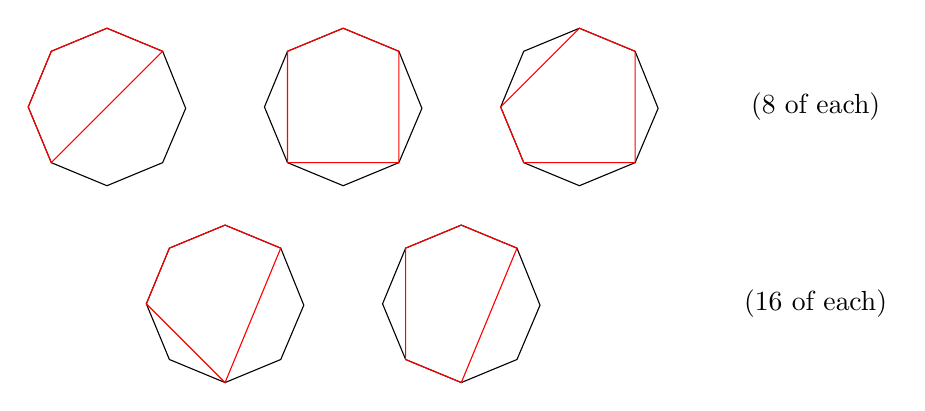
\begin{tikzpicture}
\drawOctagon
\draw[color=red] (P1) -- (P2) -- (P3) -- (P4) -- (P5) -- cycle;
\begin{scope}[xshift=3cm]
\drawOctagon
\draw[color=red] (P1) -- (P2) -- (P3) -- (P5) -- (P7) -- cycle;
\end{scope}
\begin{scope}[xshift=6cm]
\drawOctagon
\draw[color=red] (P1) -- (P2) -- (P4) -- (P5) -- (P7) -- cycle;
\end{scope}
\begin{scope}[yshift=-2.5cm,xshift=1.5cm]
\drawOctagon
\draw[color=red] (P1) -- (P2) -- (P3) -- (P4) -- (P6) -- cycle;
\end{scope}
\begin{scope}[yshift=-2.5cm, xshift=4.5cm]
\drawOctagon
\draw[color=red] (P1) -- (P2) -- (P3) -- (P5) -- (P6) -- cycle;
\end{scope}
\node[] at (9,0) (a) {(8 of each)};
\node[] at (9,-2.5) (a) {(16 of each)};
\end{tikzpicture}
\end{center}

The $A_5$ function is a sum over two of the classes of $A_2$ subalgebras, $x_2\to x_3\left(1+x_4\right)$ and $x_1 \left(1+x_2\right)\to \frac{x_2x_3}{1+x_2}$, appropriately antisymmetrized so that the overall $f_{A_5}$ picks up a minus sign under both $\sigma_{A_5}$ and $\tau_{A_5}$. Explicitly, this is written
\begin{equation}
	f_{A_5} = \sum_{i=0}^7\sum_{j=0}^1(-1)^{i+j}\sigma_{A_5}^i\tau_{A_5}^j\left(\frac12 f_{A_2}\left(x_2\to x_3\left(1+x_4\right)\right) + f_{A_2}\left(x_1 \left(1+x_2\right)\to \frac{x_2x_3}{1+x_2}\right)\right).
\end{equation}
The factor of $\frac12$ in front of $f_{A_2}\left(x_2\to x_3\left(1+x_4\right)\right)$ is simply a symmetry factor, as it lives in an 8-cycle of $\{\sigma_{A_5},\tau_{A_5}\}$.

The two types of $A_2$'s appearing in $f_{A_5}$ are:

\begin{equation}
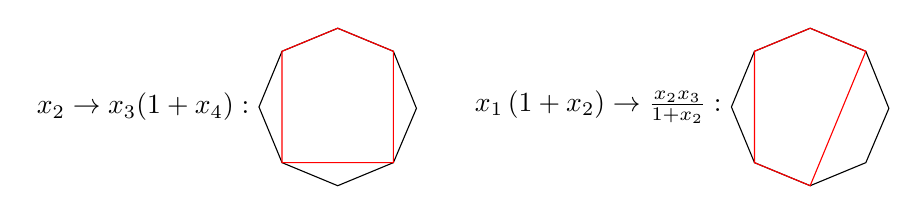
\begin{tikzpicture}
\drawOctagon
\draw[color=red] (P1) -- (P2) -- (P3) -- (P5) -- (P7) -- cycle;
\node[anchor=east] at (-1,0) (a) {$x_2 \to x_3(1+x_4):$};
\begin{scope}[xshift=6cm]
\drawOctagon
\node[anchor=east] at (-1,0) (a) {$x_1 \left(1+x_2\right)\to \frac{x_2x_3}{1+x_2}:$};
\draw[color=red] (P1) -- (P2) -- (P3) -- (P5) -- (P6) -- cycle;
\end{scope}
\end{tikzpicture}
\end{equation}

\subsection{\pdfeq{A_2\subset D_5} representation}
\subsection{\pdfeq{7\to6} collinear limits}

\section{Subalgebra representations for \pdfeq{\mathcal{P}_7^{(2)}}}

... do not seem to exist :(

\section{Tools for working with infinite cluster algebras}
\subsection{Sklyanin bracket}
In momentum twistor language we have the $n$ momentum twistors $Z_i$, which together form the $4 \times n$ matrix

\begin{equation}  
K = \left(\begin{array}{ccc}
z_{11} & \ldots & z_{n1} \\
z_{12} & \ldots & z_{n2} \\
z_{13} & \ldots & z_{n3} \\
z_{14} & \ldots & z_{n4}\end{array}\right).
\end{equation}
As long as the first 4 columns are non-singular, we can row reduce $K$ in to the form
\begin{equation}
K'=\left(
\begin{array}{ccccccc}
 1 & 0 & 0 & 0 & y_{11} & \ldots  & y_{(n-4)1} \\
 0 & 1 & 0 & 0 & y_{12} & \ldots  & y_{(n-4)2} \\
 0 & 0 & 1 & 0 & y_{13} & \ldots  & y_{(n-4)3} \\
 0 & 0 & 0 & 1 & y_{14} & \ldots  & y_{(n-4)4} \\
\end{array}
\right).
\end{equation}
The columns of $K'$ define a new set of momentum twistors $Z'_i$, where for example $Z'_1 = \{1,0,0,0\}$ and $Z'_5 = \{y_{11},y_{12},y_{13},y_{14}\}$. It is easy to check that 
\begin{align}
   &y_{ij} = (-1)^j \ket{\{1,2,3,4\}\setminus\{j\},i}/\ket{1234},\\
   &\ket{abcd}' = \det(Z'_a Z'_b Z'_c Z'_d) = \ket{abcd}/\ket{1234}.
\end{align}
You can then define the Sklyanin bracket as an operation on these $y_{ij}$ by
\begin{equation}
   \{y_{ij},y_{ab}\} = (\sgn(a-i) - \sgn(b-j)) y_{ib} y_{aj}.
\end{equation}
Which then extends to a bracket on functions of the $y_{ij}$ via
\begin{equation}\label{eq:def}
   \{f(y), g(y)\} =  \sum_{i,a=1}^n\sum_{j,b=1}^4\frac{\partial f}{\partial y_{ij}}  \frac{\partial g}{\partial y_{ab}} 
\{y_{ij}, y_{ab}\}.
\end{equation}
Now if we want to evaluate the Poisson bracket between two $\mathcal{X}$-coordinates, we can instead treat them as functions of the $y_{ij}$ and use eq.~(\ref{eq:def}). To be precise, for each four-bracket $\ket{abcd}$ in the $\mathcal{X}$-coordinates, replace them with $\ket{abcd}'$ expanded out in terms of $y_{ij}$ (e.g. $\ket{1256}' =y_{13} y_{24}-y_{14} y_{23}$). Then you can calculate eq.~(\ref{eq:def}) directly in terms of the $y_{ij}$
\subsection{Poisson/Sklyanin bracket for \pdfeq{\a}-coordinates}

\section{Identifying ``good'' variables and subalgebras in the infinite case}

In grappling with the infinite nature of the cluster algebra associated with $\Gr(4,n\ge8)$, we are guided by the knowledge of the finite subset of \acoords which will appear in the symbol of $\mathcal{E}^{(2)}_n$\cite{CaronHuot:2011ky}: 
\begin{align}\label{def:good-letters}
\begin{split}
\ket{i\,\,i{+}1\,\,jk},& \quad 
\ket{i(i{-}1\,\,i{+}1)(j\,\,j{+}1)(k\,\,k{+}1)}, \\ 
\ket{i\,\,i{+}1\,\,\bar{j}\cap\bar{k}},& \quad
\ket{i(i{-}2\,\,i{-}1)(i{+}1\,\,i{+}2)(j\,\,j{+}1)}.
\end{split}
\end{align}
We will refer to these as ``good'' \acoords. Similarly, we say an \xcoord $x$ is ``good'' if $x$ and $1+x$ are expressible as products of powers of good \acoords. In $\Gr(4,8)$ there are 116 good \acoords and 1588 good \xcoords \flag \footnote{Strictly speaking this is conjectural and has only been checked through conformal weight 16 in the numerator/denominator. It would be good to check for weight 20 \xcoords.}. Continuing the theme, within $\Gr(4,8)$ we classify subalgebras as ``good'' if they can be generated by only mutating on good \xcoords\footnote{If you mutate on good \acoords you will generate a larger class of subalgebras, as there are nodes at which there is a good \acoord but the corresponding \xcoord is not good}.

The power of these definitions is that they restrict us to a natural finite subset of $\Gr(4,n\ge8)$, and we conjecture that this subset provides all the necessary \xcoords for $\mathcal{E}^{(2)}_n$. In practice, generating good subalgebras of $\Gr(4,n)$ is accomplished by 
\begin{enumerate}
	\item generating all Pl\"ucker identities amongst good letters,
	\item this gives a list of all good \xcoords,
	\item their Poisson structure can be calculated with the Sklyanin bracket (time-consuming but finite),
	\item using the Poisson structure to identify subalgebras of interest.
\end{enumerate}
Following this procedure for $\Gr(4,8)$ gives 1600 good $A_3$ subalgebras, 496 $A_4$, 24 $D_4$, and 56 $A_5$. There are no good subalgebras larger than $A_5$. The good $A_5$ subalgebras are generated by
\begin{align}\label{eq:g48-a5s}
	&\frac{\langle 1238\rangle  \langle 1256\rangle }{\langle
   1235\rangle  \langle 1268\rangle }\to \frac{\langle
   1236\rangle  \langle 2345\rangle }{\langle 1234\rangle
    \langle 2356\rangle }\to \frac{\langle 1235\rangle 
   \langle 3456\rangle }{\langle 1356\rangle  \langle
   2345\rangle }\to \frac{\langle 1567\rangle  \langle
   2356\rangle }{\langle 1256\rangle  \langle 3567\rangle
   }\to \frac{\langle 1356\rangle  \langle 4567\rangle
   }{\langle 1567\rangle  \langle 3456\rangle },\nl
   &\frac{\langle 1238\rangle  \langle 2345\rangle
   }{\langle 1234\rangle  \langle 2358\rangle
   }\to-\frac{\langle 1235\rangle  \langle 4568\rangle
   }{\langle 5(18)(23)(46)\rangle }\to\frac{\langle
   1568\rangle  \langle 2358\rangle  \langle 3456\rangle
   }{\langle 1358\rangle  \langle 2356\rangle  \langle
   4568\rangle }\to-\frac{\langle 5(18)(23)(46)\rangle
   }{\langle 1258\rangle  \langle 3456\rangle
   }\to\frac{\langle 1278\rangle  \langle 1358\rangle
   }{\langle 1238\rangle  \langle 1578\rangle },\nl
   &\frac{\langle 1234\rangle  \langle 3456\rangle
   }{\langle 1346\rangle  \langle 2345\rangle
   }\to\frac{\langle 1348\rangle  \langle 2346\rangle
   }{\langle 1234\rangle  \langle 3468\rangle
   }\to-\frac{\langle 1346\rangle  \langle 5678\rangle
   }{\langle 6(18)(34)(57)\rangle }\to-\frac{\langle
   1678\rangle  \langle 3468\rangle  \langle 34(128)\cap
   (567)\rangle }{\langle 1268\rangle  \langle
   1348\rangle  \langle 3467\rangle  \langle 5678\rangle
   }\to\frac{\langle 1278\rangle  \langle
   6(18)(34)(57)\rangle }{\langle 1678\rangle  \langle
   34(128)\cap (567)\rangle },\nl
   &\frac{\langle 1234\rangle  \langle 1278\rangle
   }{\langle 1238\rangle  \langle 1247\rangle
   }\to-\frac{\langle 1248\rangle  \langle 3457\rangle
   }{\langle 4(12)(35)(78)\rangle }\to-\frac{\langle
   1247\rangle  \langle 12(345)\cap (678)\rangle
   }{\langle 1278\rangle  \langle 4(12)(35)(67)\rangle
   }\to-\frac{\langle 4567\rangle  \langle
   4(12)(35)(78)\rangle }{\langle 1245\rangle  \langle
   3457\rangle  \langle 4678\rangle }\to-\frac{\langle
   4(12)(35)(67)\rangle }{\langle 1234\rangle  \langle
   4567\rangle },
\end{align}
along with their symmetric images. The first $A_5$ lives in an 8-cycle of the $\Gr(4,8)$ dihedral+parity, while the other three live in 16-cycles. 

\section{Fitting the non-classical component of \pdfeq{R_8^{(2)}}}
Note that in the first $A_5$ in eq.~(\ref{eq:g48-a5s}, 7 and 8 never appear together, and so the $8\to7$ collinear limit is smooth for this $A_5$. The second $A_5$ also features a smooth collinear limit, as 
\begin{equation}
	\frac{\langle 1278\rangle  \langle 1358\rangle
   }{\langle 1238\rangle  \langle 1578\rangle } \xrightarrow{8\to7} \frac{\langle 1267\rangle  \langle 1357\rangle
   }{\langle 1237\rangle  \langle 1567\rangle }.
\end{equation}
Neither of the latter 2 $A_5$s behave smoothly in the collinear limit (and neither do any of their dihedral+parity images).

Remarkably, the $A_5$ contribution to $R^{(2)}_8$ involves simply adding together the two $A_5$'s in $\Gr(4,8)$ which behave smoothly in the collinear limit. 
\begin{equation}\label{eq:r28A5}
\begin{split}
	&R^{(2)}_8 = \frac14 f_{A_5}\left(\frac{\langle 1238\rangle  \langle 1256\rangle }{\langle
   1235\rangle  \langle 1268\rangle }\to \frac{\langle
   1236\rangle  \langle 2345\rangle }{\langle 1234\rangle
    \langle 2356\rangle }\to \frac{\langle 1235\rangle 
   \langle 3456\rangle }{\langle 1356\rangle  \langle
   2345\rangle }\to \frac{\langle 1567\rangle  \langle
   2356\rangle }{\langle 1256\rangle  \langle 3567\rangle
   }\to \frac{\langle 1356\rangle  \langle 4567\rangle
   }{\langle 1567\rangle  \langle 3456\rangle }\right)+\\
   &\frac12 f_{A_5}\left(\frac{\langle 1238\rangle  \langle 2345\rangle
   }{\langle 1234\rangle  \langle 2358\rangle
   }\to-\frac{\langle 1235\rangle  \langle 4568\rangle
   }{\langle 5(18)(23)(46)\rangle }\to\frac{\langle
   1568\rangle  \langle 2358\rangle  \langle 3456\rangle
   }{\langle 1358\rangle  \langle 2356\rangle  \langle
   4568\rangle }\to-\frac{\langle 5(18)(23)(46)\rangle
   }{\langle 1258\rangle  \langle 3456\rangle
   }\to\frac{\langle 1278\rangle  \langle 1358\rangle
   }{\langle 1238\rangle  \langle 1578\rangle }\right)\\
   &+\text{ dihedral} + \text{conjugate}
\end{split}
\end{equation}
The difference between the overall factors of the two terms is simply a result of symmetry overcounting. 


\subsection{Behavior of \pdfeq{A_5} functions in the \pdfeq{8\to7} collinear limit}
While the $A_5$'s explicitly written in (\ref{eq:r28A5}) behave smoothly under the collinear limit, not all of their dihedral+parity images do as well. In the case of the first $A_5$, which has 8 images under dihedral+parity, 4 of the $f_{A_5}$'s vanish (at the level of $\B_2 \wedge \B_2$) under the collinear limit, while the remaining 3 are non-vanishing and well-behaved. For the second $A_5$, which has 16 images under dihedral+parity, 2 of the $f_{A_5}$s have ``bad'' collinear limits but they cancel off each other in the sum. Out of the remaining 14, 4 have good collinear limits and 10 vanish identically. Therefore, when we add up the contributions from both $A_5$'s + their images, we end up with 7 terms -- these correspond to the 7 $A_5$s in $\Gr(4,7)$. 

\subsection{Behavior of \pdfeq{R_8^{(2)}} under braid automorphisms}

\section{Fitting the classical component of \pdfeq{R_8^{(2)}}}

\section{Analytic Properties of \pdfeq{R_8^{(2)}}}

\section{Steinmann relations for Eight Particles}

The Steinmann relations dictate that double discontinuities of amplitudes must vanish when taken in partially overlapping momentum channels~\cite{Steinmann,Cahill:1973qp}. It has recently been realized that these restrictions on three- (and higher-)particle channels are transparently encoded in the symbol of BDS-like normalized amplitudes when the number of scattering particles is not a multiple of four~\cite{Caron-Huot:2016owq, Dixon:2016nkn}. This follows from the fact that the BDS-like ansatz in these cases is defined to depend on just two-particle Mandelstam invariants, and thus acts as a spectator when discontinuities are taken in these channels. This subset of the Steinmann relations therefore applies directly to BDS-like-normalized amplitudes for these numbers of particles, where it implies that restricted pairs of Mandelstam invariants cannot appear sequentially in the first two entries of the symbol. In fact, these restrictions have been found to apply at all depths in the symbol, providing strong all-loop constraints on the spaces of functions that are expected to contribute to these amplitudes~\cite{omega_paper,cosmic_galois_paper}. 

More surprisingly, the extended Steinmann constraints have been found to be equivalent to demanding that every pair of sequential symbol entries appears together in some cluster in Gr(4,$n$)~\cite{Drummond:2017ssj}. In particular, it has been checked that this `cluster adjacency' principle is adhered to in all known BDS-like normalized amplitudes in six-, seven-, and nine-particle kinematics, where a unique BDS-like ansatz depending only on two-particle invariants can be defined. However, it remains less well-studied in eight-particle kinematics due to the nonexistence of any such BDS-like normalization; all eight-particle solutions to the anomalous dual conformal Ward identity governing these amplitudes in the infrared involve higher-particle Mandelstam invariants~\cite{Drummond:2007au}. For this reason, it proves necessary to explore the space of BDS-like ans\"atze that can be formed for eight particles before the (vestiges of the) Steinmann relations and cluster adjacency can be studied.

\subsection{BDS-Like Ans\"atze for Eight Particles}

\draftnote{Paragraph introducing the BDS ansatz}

When the number of particles $n$ is not a multiple of four, a unique BDS-like ansatz can be defined that depends on just two-particle Mandelstam invariants. That is, there exists just a single decomposition of the BDS ansatz into
\begin{equation}
{\cal A}_n^{\text{BDS}}(\{\mand{i,\dots,i+j}\}) = {\cal A}_n^{\text{BDS-like}}(\{\mand{i,i+1}\}) \exp \left[ - \frac{\Gamma_{\text{cusp}}}{4} Y_{n}(\{u_i\})  \right], \quad n\neq4K,
\end{equation}
such that the kinematic dependence of $A^{\text{BDS-like}}_{n}$ involves only two-particle Mandelstam invariants while $Y_{n}$ depends only on dual-conformal-invariant cross ratios~\cite{Yang:2010az}. %In particular, at one loop this relation becomes
%\begin{equation}
%A^{\text{BDS},(1)}_{n} = A^{\text{BDS-like},(1)}_{n}(\{\mand{i,i+1}\}) + Y_{n}(\{u_i\}), \quad n\neq4K,
%\end{equation}
When $n$ is a multiple of four, no decomposition of this type exists, and we are forced to consider multiple BDS-like ans\"atze if we want to transparently expose the full space of Steinmann relations between higher-particle Mandelstam invariants. 

In eight-particle kinematics, there are still two natural BDS-like normalization choices we might consider. Namely, we can let our BDS-like ansatz depend on either three- or four-particle Mandelstam invariants in addition to two-particle invariants~\cite{Dixon:2016nkn}. In this spirit, let us define a pair of BDS-like ans\"atze, respectively satisfying
\begin{align}
{\cal A}_8^{\text{BDS}}(\{\mand{i,\dots,i+j}\}) &= {}^4 {\cal A}_8^{\text{BDS-like}}(\{\mand{i,i+1}\}, \{\mand{i,i+1,i+2,i+3}\}) \exp \left[ -\frac{\Gamma_{\text{cusp}}}{4}\ {}^4 Y_{8}(\{u_i\})  \right], \label{bds_like_4} \\
%{\cal A}^{\text{BDS},(1)}_{n} &= {}^3 {\cal A}^{\text{BDS-like},(1)}_{8}(\{\mand{i,i+1}\}, \{\mand{i,i+1,i+2,i+3}\}) + {}^3 Y_{8}(\{u_i\}), \\
{\cal A}_8^{\text{BDS}}(\{\mand{i,\dots,i+j}\}) &= {}^3 {\cal A}_8^{\text{BDS-like}}(\{\mand{i,i+1}\}, \{\mand{i,i+1,i+2}\}) \exp \left[ - \frac{\Gamma_{\text{cusp}}}{4}\ {}^3 Y_{8}(\{u_i\})  \right]. \label{bds_like_3}
%{\cal A}^{\text{BDS},(1)}_{n} &= {}^4 {\cal A}^{\text{BDS-like},(1)}_{8}(\{\mand{i,i+1}\}, \{\mand{i,i+1,i+2}\}) + {}^4 Y_{8}(\{u_i\}). 
\end{align}
The functions ${}^4 A^{\text{BDS-like}}_{8}$ and ${}^3 A^{\text{BDS-like}}_{8}$ are not uniquely fixed by these decomposition choices; each admits a family of Bose-symmetric (and a larger family of non-Bose-symmetric) solutions. However, any choice for ${}^4 A^{\text{BDS-like}}_{8}$ or ${}^3 A^{\text{BDS-like}}_{8}$ consistent with eqns.~\eqref{bds_like_4} or \eqref{bds_like_3} gives rise to a BDS-like normalized amplitude that manifestly exhibits a subset of the Steinmann relations. In particular, defining
\begin{equation}
{}^X {\cal E}_8 \equiv \frac{{\cal A}_8^{\text{MHV}}}{{}^X {\cal A}^{\text{BDS-like}}_{8}} = \exp\left[ R_8 - \frac{\Gamma_{\text{cusp}}}{4} \  {}^X Y_8 \right] \label{BDS_like_amplitude}
\end{equation}
for any label $X$, we expect that ${}^4 {\cal E}_8$ should satisfy Steinmann relations between all partially overlapping pairs of three-particle invariants, while ${}^3 {\cal E}_8$ should satisfy Steinmann relations between all partially overlapping pairs of four-particle invariants. That is, ${}^4 {\cal E}_8$ is expected to satisfy the relations
\begin{equation}
\begin{split}
\text{Disc}_{\mand{j,j+1,j+2}}\left[\text{Disc}_{\mand{i,i+1,i+2}} \big({}^4 {\cal E}_8 \big) \right] &= 0, \quad  j \in \{ i \pm 2, i \pm 1 \}, \label{stein33}
\end{split}
\end{equation}
while ${}^3 {\cal E}_8$ is expected to satisfy
\begin{equation}
\begin{split}
\text{Disc}_{\mand{j,j+1,j+2,j+3}}\left[\text{Disc}_{\mand{i,i+1,i+2,i+3}} \big({}^3 {\cal E}_8 \big) \right] &= 0, \quad j \in \{ i \pm 3, i \pm 2, i \pm 1 \}.  \label{stein44}
\end{split}
\end{equation}
Due to momentum conservation in eight-point kinematics, the six relations in~\eqref{stein44} corresponding to a given $i$ only result in three independent constraints; however, these relations will be independent for larger $n$.

Although the functions ${}^4 Y_{8}$ and ${}^3 Y_{8}$ are not unique, their dilogarithmic part is completely determined by the decompositions~\eqref{bds_like_4} and~\eqref{bds_like_3}. They can be expressed as classical polylogarithms with negative arguments drawn from \begin{align}
\mathfrak{X}_{i,8} &= \frac{\langle i,i+1,i+2,i+4 \rangle \langle i+1,i+3,i+4,i+5\rangle}{\langle i,i+1,i+4,i+5 \rangle \langle i+1,i+2,i+3,i+4 \rangle}, \\
\mathfrak{X}_{i,4} &= \frac{\langle i,i+1,i+3,i+7 \rangle \langle i,i+2,i+3,i+4 \rangle}{\langle i,i+1,i+2,i+3 \rangle \langle i,i+3,i+4,i+7 \rangle},
\end{align}
where $\mathfrak{X}_{i,8}$ and $\mathfrak{X}_{i,4}$ are ${\cal X}$-coordinates in Gr(4,8) that respectively carve out an eight-orbit and a four-orbit of the dihedral group. In these variables the $\text{Li}_1$ parts of these functions can be diagonalized, giving rise to the Bose-symmetric representations
\begin{align}
{}^4 Y_8 &= \sum_{i=1}^8 \bigg[ \text{Li}_2 \left( - \mathfrak{X}_{i,8} \right) + \frac12 \text{Li}_2 \left(- \mathfrak{X}_{i,4}  \right) + \frac14 \text{Li}_1\left(- \mathfrak{X}_{i,4} \right)^2 \bigg], \\
{}^3 Y_8 &= \sum_{i=1}^8 \bigg[ \text{Li}_2 \left( - \mathfrak{X}_{i,8} \right) + \frac12 \text{Li}_2 \left(- \mathfrak{X}_{i,4}  \right) + \frac12 \text{Li}_1\left(- \mathfrak{X}_{i,8} \right)^2 \bigg].
\end{align}
We emphasize that this is an aesthetically motivated choice; there may exist other more physically (or mathematically) inspired choices that endow ${}^4 {\cal E}_8$ or ${}^3 {\cal E}_8$ with additional desirable properties. Regardless, it can be checked that any realization of ${}^4 Y_8$ or ${}^3 Y_8$ that respects Bose symmetry gives rise to a BDS-like normalized amplitude that satisfies either~\eqref{stein33} or~\eqref{stein44}, while violating all other Steinmann relations (all at the level of the symbol). 

If we want to recover more Steinmann relations, such as those holding between partially overlapping three- and four-particle invariants, we can instead define BDS-like ans\"atze that depend only on subsets of the three- or four-particle invariants. In particular, it proves possible to decompose the BDS ansatz into either
\begin{align}
{\cal A}_8^{\text{BDS}}(\{\mand{i,\dots,i+k}\}) &= {}^{{\{a,b\}}_4} {\cal A}_8^{\text{BDS-like}}(\{\mand{i,i+1}\}, \{\mand{i,i+1,i+2,i+3} | i \in \{a,b\} \})  \label{bds_like_4q} \\ 
&\hspace{5.6cm} \times \exp \left[ - \frac{\Gamma_{\text{cusp}}}{4}\ {}^{{\{a,b\}}_4} Y_{8}(\{u_i\})  \right], \nonumber  \\
{\cal A}_8^{\text{BDS}}(\{\mand{i,\dots,i+k}\}) &= {}^{{\{a,b\}}_3} {\cal A}_8^{\text{BDS-like}}(\{\mand{i,i+1}\}, \{\mand{i,i+1,i+2} | i \in \{a,b\} \})  \label{bds_like_3q} \\ 
&\hspace{5.6cm} \times \exp \left[ - \frac{\Gamma_{\text{cusp}}}{4}\ {}^{{\{a,b\}}_3} Y_{8}(\{u_i\})  \right], \nonumber 
\end{align}
for any $\{a,b\}$ such that $b-a$ is odd.\footnote{The difference $b-a$ should be computed mod 8 in the case of ${}^{{\{a,b\}}_3} {\cal A}_8^{\text{BDS-like}}$ since $\mand{i+8,\dots,i+k+8} = \mand{i,\dots,i+k}$ in general, but should be computed mod 4 in the case of ${}^{{\{a,b\}}_4} {\cal A}_8^{\text{BDS-like}}$ since momentum conservation implies the stronger identity $\mand{i+4,i+5,i+6,i+7} = \mand{i,i+1,i+2,i+3}$ between four-particle invariants.} Any solution to~\eqref{bds_like_4q} defines a BDS-like normalized amplitude $\EfourJ$ that respects the Steinmann relations
\begin{equation}
\begin{rcases}
\text{Disc}_{\mand{j,j+1,j+2}}\left[\text{Disc}_{\mand{i,i+1,i+2,i+3}} \big(\EfourJ \big) \right] \! \! \! \! &= 0, \hspace{.3cm} \\
\text{Disc}_{\mand{i,i+1,i+2,i+3}}\left[\text{Disc}_{\mand{j,j+1,j+2}} \big(\EfourJ \big) \right] \! \! \! \! &= 0, \label{stein34}
\end{rcases} \quad 
\begin{gathered} i \notin \{a,b\}, \\ j \in \{i-2, i-1, i+2, i+3\}, \end{gathered}
\end{equation}
in addition to all the Steinmann relations satisfied by ${}^4 {\cal E}_8$ as given in eq.~\eqref{stein33}. Moreover, it will respect many of the Steinmann relations satisfied by ${}^3 {\cal E}_8$---namely, those that don't involve a discontinuity in either $\mand{a,a+1,a+2,a+3}$ or $\mand{b,b+1,b+2,b+3}$. Similarly, any solution to~\eqref{bds_like_3q} defines an amplitude $\EthreeJ$ that respects
\begin{equation}
\begin{rcases}
\text{Disc}_{\mand{i,i+1,i+2}}\left[\text{Disc}_{\mand{j,j+1,j+2,j+3}} \big(\EthreeJ \big) \right] \! \! \! \! &= 0, \hspace{.3cm} \\
\text{Disc}_{\mand{j,j+1,j+2,j+3}}\left[\text{Disc}_{\mand{i,i+1,i+2}} \big(\EthreeJ \big) \right] \! \! \! \! &= 0, \label{stein43}
\end{rcases} \quad 
\begin{gathered} i \notin \{a,b\}, \\ j \in \{i-3, i-2, i+1, i+2\}, \end{gathered}
\end{equation}
%\begin{equation}
%\begin{rcases}
%\text{Disc}_{\mand{i+2,i+3,i+4}}\left[\text{Disc}_{\mand{i,i+1,i+2,i+3}} \big(\EfourJ \big) \right] \! \! \! \! &= 0, \hspace{.3cm} \\
%\text{Disc}_{\mand{i+3,i+4,i+5}}\left[\text{Disc}_{\mand{i,i+1,i+2,i+3}} \big(\EfourJ \big) \right] \! \! \! \! &= 0,  \\
%\hspace{0.324cm} \text{Disc}_{\mand{i-1,i,i+1}}\left[\text{Disc}_{\mand{i,i+1,i+2,i+3}} \big(\EfourJ \big) \right] \! \! \! \! &= 0,  \\
%\hspace{0.324cm} \text{Disc}_{\mand{i-2,i-1,i}}\left[\text{Disc}_{\mand{i,i+1,i+2,i+3}} \big(\EfourJ \big) \right] \! \! \! \! &= 0,  \\
%\text{Disc}_{\mand{i,i+1,i+2,i+3}}\left[\text{Disc}_{\mand{i+2,i+3,i+4}} \big(\EfourJ \big) \right] \! \! \! \! &= 0,  \\
%\text{Disc}_{\mand{i,i+1,i+2,i+3}}\left[\text{Disc}_{\mand{i+3,i+4,i+5}} \big(\EfourJ \big) \right] \! \! \! \! &= 0, \\
%\hspace{0.324cm} \text{Disc}_{\mand{i,i+1,i+2,i+3}}\left[\text{Disc}_{\mand{i-1,i,i+1}} \big(\EfourJ \big) \right] \! \! \! \! &= 0, \\
%\hspace{0.324cm} \text{Disc}_{\mand{i,i+1,i+2,i+3}}\left[\text{Disc}_{\mand{i-2,i-1,i}} \big(\EfourJ \big) \right] \! \! \! \! &= 0, \label{stein34}
%\end{rcases} i \notin \{a,b\}
%\end{equation}
as well as all the Steinmann relations satisfied by ${}^3 {\cal E}_8$ and described in eq.~\eqref{stein44}, and all the relations specified in eq.~\eqref{stein33} that don't involve a discontinuity in either $\mand{a,a+1,a+2}$ or $\mand{b,b+1,b+2}$. Clearly it is not possible for BDS-like amplitudes of either type to be Bose-symmetric; however, it proves possible to construct solutions to~\eqref{bds_like_3q} such that $\EthreeJ$ respects the dihedral flip $s_{i,\dots,i+k} \rightarrow s_{9-i,\dots,9-i-k}$ when this mapping is oriented to map $\mand{a,a+1,a+2}$ and $\mand{b,b+1,b+2}$ between each other. We present specific realizations of ${}^{{\{1,2\}}_4} Y_{8}$ and ${}^{{\{7,8\}}_3} Y_{8}$ in appendix~\ref{appendix:bds_like}. As with the Bose-symmetric normalization choices, it can be checked that all possible realizations of ${}^{{\{a,b\}}_4} Y_{8}$ and ${}^{{\{a,b\}}_3} Y_{8}$ give rise to BDS-like amplitudes that obey and break the same Steinmann relations (for a given pair of indices $a$ and $b$). 



\newpage

\draftnote{To Do: can any given Steinmann relation be saved (in Bose-symmetric or ...)? Any other features of the full space worth working out?}

\draftnote{To Do: define $\Gamma_{\text{cusp}}$ in this section if we don't earlier}

\draftnote{To Do: comment about the fact that we don't know how to extend the Steinmann relations beyond symbol level (or figure out how to do so...)}

\subsection{Restoring all Steinmann Relations}

\draftnote{To Do: discuss the possibility of repairing Steinmann and cluster adjacency at the cost of dual conformal invariance, and also in special kinematic limits where the additional three- or four-particle dependence drops out}

\section{Conclusion}

\appendix

\section{BDS-Like Conversions for Eight Particles} \label{appendix:bds_like}

 \begin{align}
{}^{{\{1,2\}}_4} Y_{8} &= {}^{4}Y_8 -
\Big( \LiOneCalX{1}{4} + \LiOneCalX{4}{4} + \LiOneCalX{4}{8} + \LiOneCalX{8}{8} \Big)  \\
&\hspace{3.4cm} \times \Big( \LiOneCalX{3}{4}+ \LiOneCalX{4}{4} + \LiOneCalX{3}{8} + \LiOneCalX{7}{8} \Big) \nonumber
\end{align}

 \begin{align}
{}^{{\{7,8\}}_3} Y_{8} &= \sum_{i=1}^8 \bigg[ \text{Li}_2 \left( - \mathfrak{X}_{i,8} \right) + \frac12 \text{Li}_2 \left(- \mathfrak{X}_{i,4}  \right) + \frac14 \text{Li}_1\left(- \mathfrak{X}_{i,4} \right)^2 \bigg] \nonumber \\
&\hspace{.4cm}- \bigg[ \frac 12\Big( \LiOneCalX{1}{4} + \LiOneCalX{3}{4} \Big) \Big( \LiOneCalX{2}{4} + \LiOneCalX{4}{4} \Big)  \nonumber \\
&\hspace{1.2cm} + \LiOneCalX{1}{4}  \Big( \LiOneCalX{1}{8} + \LiOneCalX{4}{8} + \LiOneCalX{6}{8} + \LiOneCalX{7}{8} \Big) \nonumber \\ 
&\hspace{1.2cm} + \LiOneCalX{2}{4}  \Big( \LiOneCalX{1}{8} + \LiOneCalX{4}{8} - \LiOneCalX{6}{8}  -  \LiOneCalX{3}{8} \Big) \\
&\hspace{1.2cm} + \LiOneCalX{1}{8}  \Big( \LiOneCalX{4}{8} + \frac12  \LiOneCalX{1}{8} - \frac12 \LiOneCalX{3}{8} \Big) \nonumber \\
&\hspace{1.2cm} + \LiOneCalX{5}{8}  \Big( \LiOneCalX{4}{8} - \frac12  \LiOneCalX{5}{8} + \frac12 \LiOneCalX{7}{8} \Big) \nonumber \\
&\hspace{1.2cm} + \LiOneCalX{6}{8}  \Big( \LiOneCalX{4}{8} - \frac12  \LiOneCalX{2}{8} - \frac12 \LiOneCalX{6}{8} \Big)\nonumber \\
&\hspace{1.2cm} - \LiOneCalX{2}{4} \LiOneCalX{3}{4} \bigg]_{\LiOneCalX{i}{j} + \LiOneBarCalX{i}{j}} \nonumber
\end{align}
where $\overline{\mathfrak{X}}_{i,j}$ is the image of the ${\cal X}$-coordinate $\mathfrak{X}_{i,j}$ under the dihedral flip that sends $Z_i \rightarrow Z_{9-i}$ (that is, the expression in the second square bracket is understood to be the sum of itself and this dihedral image). 


The decompositions~\eqref{bds_like_3}, \eqref{bds_like_4}, and \eqref{bds_like_3q} do not uniquely determine ${}^{3} Y_{8}$, ${}^{4} Y_{8}$, or ${}^{3,j} Y_{8}$. In fact, there exists a 10-dimensional (3-dimensional) space of (Bose-symmetric) solutions for ${}^{3} Y_{8}$, a 36-dimensional (5-dimensional) space of (Bose-symmetric) solutions for ${}^{4} Y_{8}$, and a 3-dimensional space of solutions for ${}^{3,j} Y_{8}$. 
 \begin{align}
{}^{3,1}Y_8 &= {}^{3}Y_8 -
\Big( \text{Li}_1(-\mathfrak{X}_{1, 4}) + \text{Li}_1(-\mathfrak{X}_{2, 4}) + \text{Li}_1(-\mathfrak{X}_{1, 8}) + \text{Li}_1(-\mathfrak{X}_{5, 8}) \Big)  \\
&\hspace{3.4cm} \times \Big( \text{Li}_1(-\mathfrak{X}_{1, 4}) + \text{Li}_1(-\mathfrak{X}_{4, 4}) + \text{Li}_1(-\mathfrak{X}_{4, 8}) + \text{Li}_1(-\mathfrak{X}_{8, 8}) \Big) \nonumber
\end{align}

 \begin{align*}
 &\ \hspace{1.4cm}- \log(s_{\scaleto{1234}{4.4pt}} s_{\scaleto{3456}{4.4pt}}) \log(s_{\scaleto{2345}{4.4pt}} s_{\scaleto{4567}{4.4pt}}) \nonumber
 \end{align*}
 
 \begin{align*}
&\ \hspace{2.4cm}- \frac12 \log(\mand{i,i+1,i+2}) \log\left(\frac{\mand{i,i+1,i+2} \ \mand{i+1,i+2,i+3}^2}{\mand{i+4,i+5,i+6}}\right) \bigg] \nonumber
 \end{align*}
 
 To take full advantage of the Steinmann relations, it is convenient to work in terms of symbol letters that isolate different Mandelstam invariants. There are twelve independent dual conformally invariant cross ratios that can appear in these symbols
\begin{align}
u_1 &= \frac{\mand{12} \mand{4567}}{\mand{123} \mand{812}}, \quad \text{and cyclic (8-orbit)} \\
u_9 &= \frac{\mand{123} \mand{567}}{\mand{1234} \mand{4567}}, \quad \text{and cyclic (4-orbit).}
\end{align}
It is not possible to isolate all three- and four-particle Mandelstam invariants simultaneously into twelve different symbol letters. (More than twelve symbol letters will appear in these amplitudes, but we here restrict our attention to the twelve that will appear in the first entry.) However, different choices of letters can be made such that either all the four-particle invariants, or all the three-particle invariants, are isolated.

One choice that isolates the four-particle invariants is
\begin{align}
{}^4 d_1 &= u_2 \ u_6 = \frac{\mand{23} \ \mand{67} \ (\mand{1234})^2}{\mand{123} \ \mand{234} \ \mand{567} \ \mand{678}}, \quad \text{and cyclic (4-orbit)} \\
{}^4 d_5 &= u_2/u_6 = \frac{\mand{23} \ \mand{567} \ \mand{678}}{\mand{67} \ \mand{123} \ \mand{234}}, \quad \text{and cyclic (4-orbit)} \\
{}^4 d_9 &= u_1 \ u_2 \ u_5 \ u_6 \ u_9^2 = \frac{\mand{12} \ \mand{23} \ \mand{56} \ \mand{67}}{\mand{234} \ \mand{456} \ \mand{678} \ \mand{812}}, \quad \text{and cyclic (4-orbit)}.
\end{align}
In this alphabet ${}^4 d_1, {}^4 d_2, {}^4 d_3$, and ${}^4 d_4$ each contain a different four-particle Mandelstam invariant, while the other letters only involve two- and three-particle invariants. The extended Steinmann relations then tell us that ${}^4 d_1, {}^4 d_2, {}^4 d_3$, and ${}^4 d_4$ can never appear next to each other in the symbol of ${}^4 A^{\text{BDS-like}}_{8}$ (but each can still appear next to themselves).

Similarly, we can isolate the three-particle invariants by choosing
\begin{align}
{}^3 d_1 &= \frac{u_1 \ u_2 \ u_4 \ u_7}{u_3 \ u_5 \ u_6 \ u_8 \ u_9^2} = \frac{\mand{12} \ \mand{23} \ \mand{45} \ \mand{78} \ (\mand{1234})^2 \ (\mand{4567})^2}{\mand{34} \ \mand{56} \ \mand{67} \ \mand{81} \ (\mand{123})^2}, \quad \text{and cyclic (8-orbit)} \\
{}^3 d^4_9 &= u_1 \ u_5 \ u_9 \ u_{12} = \frac{\mand{12} \ \mand{56}}{\mand{1234} \ \mand{3456}}, \quad \text{and cyclic (4-orbit)},
\end{align}
in which case ${}^3 d_1$ through ${}^3 d_8$ each contain a different three-particle Mandelstam invariant, as well as four-particle Mandelstams that they don't partially overlap with. The remaining four letters only contain two- and four-particle invariants. In these letters, conditions~\eqref{stein34_5} and~\eqref{stein34_6} tell us that ${}^3 d_7, {}^3 d_8, {}^3 d_2$, and ${}^3 d_3$ can never appear next to ${}^3 d_1$ in the symbols of ${}^{3} {\cal E}_8$ or ${}^{3,j} {\cal E}_8$ (plus the cyclic images of this statement). Moreover, conditions~\eqref{stein34_1} through~\eqref{stein34_4} give us the additional restrictions that none of ${}^3 d_1, {}^3 d_5, {}^3 d_9$ and ${}^3 d_{10}$ can ever appear next to ${}^3 d_3, {}^3 d_4, {}^3 d_7,$ or ${}^3 d_8$ in the symbol of ${}^{3,1} {\cal E}_8$ (analogous relations hold for the other ${}^{3,j} {\cal E}_8$). These are the restrictions given by the Steinmann relations involving $\mand{1234}$ and one of $\mand{781}, \mand{812}, \mand{345}$, or $\mand{456}$. The other Steinmann relations between three- and four-particle invariants will not be respected by ${}^{3,1} {\cal E}_8$, since ${}^{3,j} {\cal A}^{\text{BDS-like}}_{8}$ depends on $\mand{2345}, \mand{3456},$ and $\mand{4567}$.

\bibliographystyle{ieeetr}

\bibliography{subalgebras.bib}

\end{document}
